\documentclass[11pt,twoside,a4paper]{article}
% http://www-h.eng.cam.ac.uk/help/tpl/textprocessing/latex_maths+pix/node6.html symboles de math
% http://fr.wikibooks.org/wiki/Programmation_LaTeX Programmation latex (wikibook)
%=========================== En-Tete =================================
%--- Insertion de paquetages (optionnel) ---
\usepackage[french]{babel}   % pour dire que le texte est en fran{\'e}ais
\usepackage{a4}	             % pour la taille   
\usepackage[T1]{fontenc}     % pour les font postscript
\usepackage{epsfig}          % pour gerer les images
%\usepackage{psfig}
\usepackage{amsmath, amsthm} % tres bon mode mathematique
\usepackage{amsfonts,amssymb}% permet la definition des ensembles
\usepackage{float}           % pour le placement des figure
\usepackage{verbatim}

\usepackage{longtable} % pour les tableaux de plusieurs pages

\usepackage[table]{xcolor} % couleur de fond des cellules de tableaux

\usepackage{lastpage}

% \usepackage[top=1.5cm, bottom=1.5cm, left=1.5cm, right=1.5cm]{geometry}
% gauche, haut, droite, bas, entete, ente2txt, pied, txt2pied
\usepackage{vmargin}
\setmarginsrb{1.00cm}{1.00cm}{1.00cm}{1.00cm}{15pt}{3pt}{15pt}{3pt}

\usepackage{lscape} % changement orientation page
%\usepackage{frbib} % enlever pour obtenir references en anglais
% --- style de page (pour les en-tete) ---
\pagestyle{empty}

% % % en-tete et pieds de page configurables : fancyhdr.sty

% http://www.trustonme.net/didactels/250.html

% http://ww3.ac-poitiers.fr/math/tex/pratique/entete/entete.htm
% http://www.ctan.org/tex-archive/macros/latex/contrib/fancyhdr/fancyhdr.pdf
% \usepackage{fancyhdr}
% \pagestyle{fancy}
% % \newcommand{\chaptermark}[1]{\markboth{#1}{}}
% % \newcommand{\sectionmark}[1]{\markright{\thesection\ #1}}
% \fancyhf{}
% \fancyhead[LE,RO]{\bfseries\thepage}
% \fancyhead[LO]{\bfseries\rightmark}
% \fancyhead[RE]{\bfseries\leftmark}
% \fancyfoot[LE]{\thepage /\pageref{LastPage} \hfill
	% TITLE
% \hfill 
\includegraphics[width=0.5cm]{img/logo_glider.png} }
% \fancyfoot[RO]{
\includegraphics[width=0.5cm]{img/logo_glider.png} \hfill
	% TITLE
% \hfill \thepage /\pageref{LastPage}}
% \renewcommand{\headrulewidth}{0.5pt}
% \renewcommand{\footrulewidth}{0.5pt}
% \addtolength{\headheight}{0.5pt}
% \fancypagestyle{plain}{
	% \fancyhead{}
	% \renewcommand{\headrulewidth}{0pt}
% }

\usepackage{lettrine}
\usepackage{fancybox}

%============================= Corps =================================
\begin{document}

\setlength\parindent{0pt}

%% \texttt{  }~\\

%% \textbf{\LARGE }~\\

%% \emph{\small }~\\

%% \begin{minipage}[ht]{0.75\textwidth}
%% 	~\\
%% \end{minipage} \hfill \begin{minipage}[ht]{6.15cm}
%% 	\includegraphics[width=6.00cm]{img/*****}
%% \end{minipage}~\\~\\

\clearpage

\texttt{http://www.journaldugeek.com/2012/06/12/flame-un-lien-de-parente-avec-stuxnet/}~\\

\textbf{\LARGE Flame, un lien de parent{\'e} avec Stuxnet ?}~\\

\textbf{\small Par Pierre, 12 juin 2012 {\`a} 10:50}~\\

\begin{minipage}[ht]{6.25cm}	
	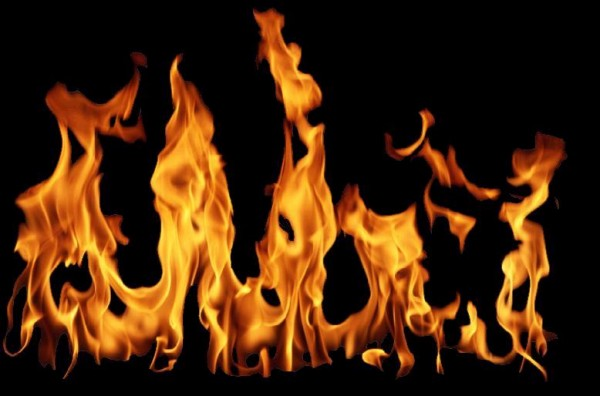
\includegraphics[width=6.00cm]{img/13ae95fb1-600x396.jpg}
\end{minipage} \hfill \begin{minipage}[ht]{12.50cm}
	\small
	M{\^e}me apr{\`e}s son suicide~\footnotemark, Flame continue d'{\^e}tre au centre des attentions des soci{\'e}t{\'e}s de s{\'e}curit{\'e}. Kapersky continue ses investigations sur la cyberarme, et d{\'e}clare avoir d{\'e}couvert que Flame aurait des \textbf{liens forts avec le malware Stuxnet}. Kapersky aurait d{\'e}couvert que Flame serait ant{\'e}rieur {\`a} Stuxnet, et que ce dernier aurait en grande partie le m{\^e}me code source que son grand fr{\`e}re.~\\
	
	Flame, d{\'e}couvert il y a peu, serait en activit{\'e} depuis 2008, toujours selon Kapersky, et les cr{\'e}ateurs des deux malwares auraient travaill{\'e} ensemble au moins une fois aux premiers stades de d{\'e}veloppement.~\\
\end{minipage}~\\
~\footnotetext{http://www.journaldugeek.com/2012/06/08/flame-le-malware-passe-en-mode-autodestruction/}

Les deux programmes auraient donc \textbf{la m{\^e}me origine}, selon Kapersky. Le \emph{New York Times~\footnote{\texttt{http://www.nytimes.com/2012/06/01/world/middleeast/obama-ordered-wave-of-cyberattacks-against-iran.html?\_r=2\&pagewanted=1}}} pr{\'e}cise lui que Stuxnet, apparu en 2009 pour cibler les ordinateurs d'une usine d'enrichissement d'uranium Iranien, aurait {\'e}t{\'e} d{\'e}velopp{\'e} et utilis{\'e} par l'\textbf{agence de s{\'e}curit{\'e} nationale des {\'E}tats-Unis}, sous l'{\`e}re Bush, puis sous Obama. Des informaticiens Isra{\'e}liens seraient {\'e}galement impliqu{\'e}s dans son d{\'e}veloppement.~\\

Flame, qui s'est autod{\'e}truit la semaine derni{\`e}re, vraisemblablement pour ne pas que l'on d{\'e}couvre ses origines, aurait donc \textbf{peut-{\^e}tre failli {\`a} sa mission}. Flame est la plus grosse cyberarme jamais con\c{c}ue, selon Kapersky, et {\'e}tait destin{\'e}e au cyber espionnage. Stuxnet, lui, avait {\'e}t{\'e} con\c{c}u pour des missions de sabotage.~\\

\texttt{Source~\footnote{\texttt{http://www.lemonde.fr/technologies/article/2012/06/11/les-virus-informatiques-flame-et-stuxnet-seraient-lies\_1716742\_651865.html}}}~\\

%% \clearpage

\texttt{http://www.lemonde.fr/technologies/article/2012/06/11/les-virus-informatiques-flame-et-stuxnet-seraient-lies\_1716742\_651865.html}~\\

\textbf{\LARGE Les virus informatiques Flame et Stuxnet seraient li{\'e}s}~\\

\textbf{\small Le Monde.fr avec AFP | 11.06.2012 {\`a} 21h41}~\\

Le virus informatique Flame, une cyberarme notamment con\c{c}ue pour d{\'e}rober des documents du programme nucl{\'e}aire iranien, pr{\'e}sente des liens avec Stuxnet, un logiciel qui s'en {\'e}tait {\'e}galement pris {\`a} T{\'e}h{\'e}ran, a affirm{\'e} lundi 11 juin la soci{\'e}t{\'e} de s{\'e}curit{\'e} informatique russe Kaspersky.~\\

Alexander Gostev, un sp{\'e}cialiste de la soci{\'e}t{\'e} russe, indique dans un blog qu'une premi{\`e}re analyse avait montr{\'e} que les deux programmes n'{\'e}taient pas li{\'e}s. "\emph{Mais il s'est av{\'e}r{\'e} que nous avions tort}", dit-il. "\emph{Nos recherches ont r{\'e}v{\'e}l{\'e} certaines informations qui changent compl{\`e}tement la mani{\`e}re dont nous pensions que Stuxnet a {\'e}t{\'e} cr{\'e}{\'e} et ses liens avec Flame}".~\\

Cette affirmation intervient juste apr{\`e}s que la soci{\'e}t{\'e} am{\'e}ricaine de s{\'e}curit{\'e} informatique Symantec a affirm{\'e} dimanche sur son blog que Flame avait re\c{c}u l'ordre de dispara{\^i}tre sans laisser de trace.~\\

~\\

\textbf{\large DEUX {\'E}QUIPES DE PROGRAMMATEURS}~\\

Bien que d{\'e}couvert plus r{\'e}cemment, Flame serait ant{\'e}rieur {\`a} Stuxnet, cr{\'e}{\'e} en 2009, a poursuivi M. Gostev. "\emph{Le code de Stuxnet utilise une structure de programmation con\c{c}ue sur Flame et probablement d{\'e}velopp{\'e}e sp{\'e}cifiquement pour fonctionner avec Stuxnet}". Cela sugg{\`e}re l'existence de "\emph{deux {\'e}quipes de programmateurs ind{\'e}pendantes}", li{\'e}es entre elles, et "\emph{travaillant chacune sur sa propre plateforme depuis 2007-2008 au plus tard}", a-t-il ajout{\'e}, pr{\'e}cisant que Flame pourrait dater de l'{\'e}t{\'e} 2008.~\\

Le virus Flame a {\'e}t{\'e} d{\'e}tect{\'e} dans diff{\'e}rentes r{\'e}gions du monde, notamment le Moyen-Orient, l'Europe, l'Am{\'e}rique du Nord et l'Asie-Pacifique, l'Iran {\'e}tant le premier pays vis{\'e} par des attaques. Le ministre isra{\'e}lien des affaires strat{\'e}giques, Mosh{\'e} Yaalon, a justifi{\'e} r{\'e}cemment le recours {\`a} de puissants virus informatiques afin de contrer la menace nucl{\'e}aire iranienne, alimentant les sp{\'e}culations sur une possible implication d'Isra{\"e}l dans ce programme informatique. Flame existait depuis quatre ans, mais il n'avait {\'e}t{\'e} identifi{\'e} que fin mai par Kaspersky, qui avait not{\'e} que la sophistication de ce virus utilis{\'e} {\`a} des fins de "cyberespionnage" {\'e}tait telle qu'il supposait le concours d'un Etat.~\\

%% \clearpage

\texttt{http://www.01net.com/editorial/568111/cyberguerre-kasperksy-etablit-le-lien-entre-stuxnet-et-flame/}~\\

\textbf{\LARGE Cyberguerre : Kasperksy {\'e}tablit le lien entre Stuxnet et Flame}~\\

\textbf{\small Eric le Bourlout -- 01net -- le 11/06/12 {\`a} 19h00}~\\

\textbf{L'entreprise russe indique que le kit d'espionnage et Stuxnet partagent un module en commun, ce qui prouverait que les {\'e}quipes qui ont con\c{c}u ces deux malwares ont collabor{\'e}.}~\\

\begin{minipage}[ht]{6.25cm}	
	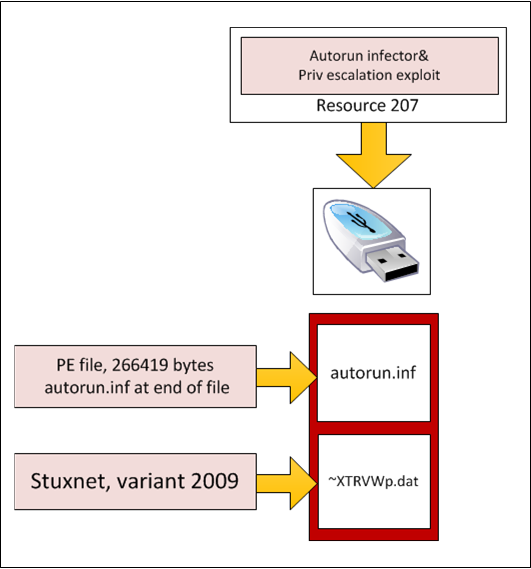
\includegraphics[width=6.00cm]{img/686461.png}
	~\\ \emph{\small Un des modules de Flame utilise le m{\^e}me code qu'une ancienne version de Stuxnet pour une infection par USB}
\end{minipage} \hfill \begin{minipage}[ht]{12.50cm}
	\small
	Deux malwares, une m{\^e}me {\'e}quipe ? La firme de s{\'e}curit{\'e} russe Kaspersky \texttt{vient de d{\'e}montrer~\footnotemark} que Stuxnet et Flame avaient des points communs qui n'avaient pas {\'e}t{\'e} rep{\'e}r{\'e}s lors des premi{\`e}res analyses. Kaspersky avait en effet indiqu{\'e} qu'il s'agissait de deux projets parall{\`e}les, cod{\'e}s tr{\`e}s diff{\'e}remment, qui ne semblaient donc pas avoir d'auteurs communs.~\\
	
	Mais apr{\`e}s avoir {\'e}tudi{\'e} Flame, et en particulier un des nombreux modules de celui-ci avec attention, Kaspersky a revu son jugement et est d{\'e}sormais certain qu'il existe au moins un lien entre les cr{\'e}ateurs de Stuxnet et de Flame.~\\  

	Leur d{\'e}couverte concerne un bout de code sp{\'e}cifique de la premi{\`e}re version de Stuxnet -- qui remonte {\`a} 2009 : on y retrouve en effet un module baptis{\'e} << Resource 207 >> qui a ensuite {\'e}t{\'e} fondu dans d'autres modules dans les versions suivantes du ver. << \emph{Resource 207 est un fichier DLL crypt{\'e}, et cachant un ex{\'e}cutable nomm{\'e} atmpsvcn.ocx [...]. Ce fichier particulier [...] pr{\'e}sente de nombreux points communs avec le code utilis{\'e} dans Flame. Parmi ces ressemblances frappantes figurent des noms d'objets identiques, l'algorithme de d{\'e}cryptage employ{\'e} ainsi que des m{\'e}thodes similaires d'attribution des noms de fichiers } >>, indique Kaspersky dans un communiqu{\'e}.~\\
\end{minipage}~\\
~\footnotetext{\texttt{http://www.securelist.com/en/blog/208193568/Back\_to\_Stuxnet\_the\_missing\_link}}

\textbf{\large Resource 207, un des modules de Flame}~\\

La firme pr{\'e}cise que cette Resource 207 n'est ni plus ni moins qu'un des modules de Flame. Il sert {\`a} propager l'infection d'une machine {\`a} l'autre via une cl{\'e} USB. C'{\'e}tait l'un des moyens de propagation principaux de Stuxnet et reposait {\`a} l'{\'e}poque sur une faille zero-day, corrig{\'e}e depuis par Microsoft.~\\

D'apr{\`e}s Kaspersky, cela prouve plusieurs choses. Non seulement que les auteurs de Stuxnet et de Flame sont li{\'e}s : ils ont collabor{\'e} et partag{\'e} ce module pr{\'e}cis. Mais cette d{\'e}couverte montre aussi que Flame est ant{\'e}rieur {\`a} Stuxnet, puisque Kaspersky estime la cr{\'e}ation de l'outil d'espionnage {\`a} l'{\'e}t{\'e} 2008, alors que Stuxnet a vu le jour en 2009. Les auteurs de Stuxnet auraient simplement r{\'e}cup{\'e}r{\'e} un des modules de Flame pour am{\'e}liorer la cyberarme destin{\'e}e {\`a} frapper les installations nucl{\'e}aires iraniennes.~\\

Kaspersky indique toutefois que si les {\'e}quipes ont partag{\'e} le code source d'un module, les deux codes malveillants demeurent tr{\`e}s distincts dans leur programmation, ce qui signifierait qu'ils ont {\'e}t{\'e} programm{\'e}s par des {\'e}quipes diff{\'e}rentes, se retrouvant ponctuellement pour partager certains de leurs programmes.~\\

Ces r{\'e}v{\'e}lations pourraient avoir des r{\'e}percussions importantes sur le plan international : il y a quelques jours, le New York Times r{\'e}v{\'e}lait que Stuxnet avait {\'e}t{\'e} d{\'e}velopp{\'e} sur ordre de l'administration Bush et qu'Isra{\"e}l avait contribu{\'e} {\`a} sa conception.%% ~\\

\clearpage

\texttt{http://www.linformaticien.com/actualites/id/25172/flame-des-liens-avec-stuxnet.aspx}~\\

\textbf{\LARGE Flame : des liens avec Stuxnet}~\\

\textbf{\small par St{\'e}phane Larcher, le 11 juin 2012 16:15}~\\

Kaspersky poursuit son {\'e}tude du virus Flame lequel est en phase d'autodestruction et met en {\'e}vidence l'existence d'un lien entre les d{\'e}veloppeurs de Stuxnet et ceux de Flame.~\\

Flame n'a pas fini de livrer tous ces secrets. Et ceux-ci seront peut-{\^e}tre difficiles {\`a} tous trouver car le programme malveillant est entr{\'e} dans une phase de suicide sur les postes sur lesquels il {\'e}tait install{\'e}, une preuve suppl{\'e}mentaire - s'il en {\'e}tait besoin -  de la tr{\`e}s grande sophistication de ce programme, une caract{\'e}ristique imm{\'e}diatement d{\'e}cel{\'e}e par l'{\'e}diteur russe.~\\

Alexandre Kostev, l'un des principaux chercheurs de virus, poursuit ses investigations et vient de d{\'e}couvrir un lien entre les d{\'e}veloppeurs de Stuxnet et de Flame. A un moment o{\`u} viennent d'{\^e}tre r{\'e}v{\'e}l{\'e}es les tribulations am{\'e}ricaines en mati{\`e}re de cyberguerre, cette d{\'e}couverte renforce l'id{\'e}e que ce programme a {\'e}t{\'e} d{\'e}velopp{\'e} par un Etat, vraisemblablement les Etats-Unis.  Dans un ouvrage paru tr{\`e}s r{\'e}cemment, un journaliste du New York Times, extr{\^e}mement bien inform{\'e}, a mis en lumi{\`e}re le r{\^o}le de l'Administration Obama dans la poursuite voire le d{\'e}veloppement de programmes de cyberguerre {\`a} l'encontre de l'Iran et en partenariat avec Isra{\"e}l dans le cadre de Stuxnet.~\\

\textbf{\large Un module de Stuxnet est un plugin de Flame}~\\

Dans sa derni{\`e}re publication, Kaspersky Lab a d{\'e}couvert qu'un module de la version de Stuxnet de d{\'e}but 2009, connu sous le nom << Resource 207 >>, se trouve {\^e}tre aussi un plugin de Flame. Cela signifie que, lors de la cr{\'e}ation du ver Stuxnet d{\'e}but 2009, la plate-forme Flame existait d{\'e}j{\`a} et que, d{\`e}s 2009, le code source d'au moins un module de Flame a {\'e}t{\'e} utilis{\'e} dans Stuxnet. Ce module, servant {\`a} propager l'infection via des cl{\'e}s USB, pr{\'e}sente un m{\'e}canisme identique dans Flame et Stuxnet. Le module Flame dans Stuxnet exploitait {\'e}galement une vuln{\'e}rabilit{\'e} inconnue {\`a} l'{\'e}poque et permettant aussi d'atteindre les autorisations d'acc{\`e}s les plus {\'e}lev{\'e}es dans la hi{\'e}rarchie (sans doute MS09-025). Par la suite, le module Flame a {\'e}t{\'e} retir{\'e} de Stuxnet en 2010 et remplac{\'e} par diff{\'e}rents autres mettant {\`a} profit de nouvelles vuln{\'e}rabilit{\'e}s. A partir de 2010, les deux {\'e}quipes de d{\'e}veloppement ont travaill{\'e} chacune de leur c{\^o}t{\'e}, leur seule coop{\'e}ration suppos{\'e}e consistant {\`a} {\'e}changer leur savoir-faire sur les nouvelles failles << zero day >>.~\\ 

Les explications compl{\`e}tes fournies par M. Kostev sont accessibles {\`a} cette \textbf{adresse~\footnote{\texttt{http://www.securelist.com/en/blog/208193568/Back\_to\_Stuxnet\_the\_missing\_link}}}. ~\\

%% \clearpage

\texttt{http://www.01net.com/editorial/567735/flame-les-premiers-secrets-de-la-cyberarme-reveles/}~\\

\textbf{\LARGE Flame : les premiers secrets de la cyberarme r{\'e}v{\'e}l{\'e}s}~\\

\textbf{\small Eric le Bourlout -- 01net -- le 07/06/12 {\`a} 17h27}~\\

\textbf{Les d{\'e}tails sur le fonctionnement de Flame commencent {\`a} tomber. Le logiciel malveillant, analys{\'e} notamment par les {\'e}quipes de Kaspersky et de Symantec, est bel et bien incroyablement complexe... et r{\'e}serve quelques surprises.}~\\ 

Percer les secrets de Flame, le puissant kit d'espionnage d{\'e}masqu{\'e} r{\'e}cemment, sera un travail de tr{\`e}s longue haleine. Mais les experts en s{\'e}curit{\'e} qui proc{\`e}dent {\`a} son analyse ont d{\'e}j{\`a} d{\'e}cortiqu{\'e} certains de ses principes de fonctionnement. Et ce qu'ils ont d{\'e}couvert corrobore la th{\'e}orie selon laquelle ce logiciel malveillant serait l'un des plus avanc{\'e}s au monde.~\\

\begin{minipage}[ht]{6.25cm}	
	
\includegraphics[width=6.00cm]{img/685315.jpg}
\end{minipage} \hfill \begin{minipage}[ht]{12.50cm}
	\small
	Kaspersky, \texttt{qui a r{\'e}v{\'e}l{\'e} l'existence de Flame~\footnotemark}, est en pointe sur l'{\'e}tude du malware. La firme de s{\'e}curit{\'e} russe d{\'e}taille sur son blog l'\texttt{avancement de ses recherches~\footnotemark} et donne quelques d{\'e}tails int{\'e}ressants {\`a} son propos, {\`a} commencer par une description des modules qui le composent. Alexander Gostev, chercheur au sein de Kaspersky, {\'e}voque aussi le nom du fichier principal de Flame, MSSECMGR.OCX, dont une des versions d{\'e}couvertes p{\`e}se pas moins de 6 Mo !~\\
	
	Pourquoi une taille aussi importante ? Parce que ce fichier abrite diff{\'e}rents modules, pour certains tr{\`e}s complexes, qui permettent {\`a} Flame d'espionner, de se r{\'e}pandre ou de communiquer avec ses myst{\'e}rieux ma{\^i}tres. Kaspersky n'est pas encore parvenu {\`a} comprendre l'utilit{\'e} de chacun d'entre eux, mais d{\'e}voile tout de m{\^e}me de nombreuses informations croustillantes.~\\
\end{minipage}
~\footnotetext{\texttt{http://www.01net.com/editorial/567055/flame-la-plus-sophistiquee-des-cyberarmes/}}
~\footnotetext{\texttt{http://www.securelist.com/en/blog}}

\begin{minipage}[ht]{12.50cm}
	Pour n'en citer que quelques unes : << Beetlejuice >> permet, par exemple, {\`a} Flame d'utiliser le Bluetooth pour faire un rep{\'e}rage des appareils pr{\'e}sents autour de la machine infect{\'e}e. << Microbe >> offre la possibilit{\'e} d'enregistrer des sons {\`a} partir du micro. Quant {\`a} << Limbo >>, il cr{\'e}e de nouveaux comptes masqu{\'e}s sur les machines pr{\'e}sentes sur le m{\^e}me r{\'e}seau que le PC infect{\'e}, pour les contaminer ensuite gr{\^a}ce {\`a} un autre module : << Frog >>.~\\
	
	Le spectre des donn{\'e}es collect{\'e}es est impressionnant. Symantec en a dress{\'e} \texttt{une liste proprement incroyable~\footnotemark}... D'apr{\`e}s ses informations, l'espion est capable de r{\'e}cup{\'e}rer {\`a} peu pr{\`e}s tout ce qui se trouve sur la machine, des donn{\'e}es syst{\`e}me aux flux r{\'e}seau, en passant par les mots de passe et les fichiers qui y sont stock{\'e}s (\emph{voir notre image}) !~\\
	
	\textbf{\large Flame peut se r{\'e}pandre via Windows Update}~\\

	Autre preuve de l'intelligence, de l'ing{\'e}niosit{\'e} des d{\'e}veloppeurs de Flame : sa capacit{\'e} {\`a} se propager, {\`a} la demande de ses ma{\^i}tres, de nombreuses mani{\`e}res. Deux autres modules, que Kaspersky nomme << Gadget >> et << Munch >> profitent notamment d'une technique particuli{\`e}rement maline pour r{\'e}pandre discr{\`e}tement le kit d'espionnage sur diff{\'e}rents PC d'un m{\^e}me r{\'e}seau local. Et pas grand-chose ne peut lui r{\'e}sister, pas m{\^e}me un PC << patch{\'e} >> avec les derniers correctifs.~\\
	
	L'attaque, particuli{\`e}rement originale, consiste en effet {\`a} d{\'e}guiser le code malveillant en... une mise {\`a} jour Windows Update. Pour cela, Flame fait passer la machine initialement infect{\'e}e pour un proxy du service de mise {\`a} jour. Quand la machine cible se connecte {\`a} Windows Update, elle est redirig{\'e}e {\`a} l'insu de l'utilisateur sur l'ordinateur d{\'e}j{\`a} infect{\'e}. Celui-ci va alors servir une fausse mise {\`a} jour Windows : << Desktop Gadget Platform >>, cens{\'e}e permettre l'affichage de widgets sur le bureau. Il n'en est rien : c'est bien Flame qui est install{\'e} !~\\
\end{minipage} \hfill \begin{minipage}[ht]{6.25cm}	
	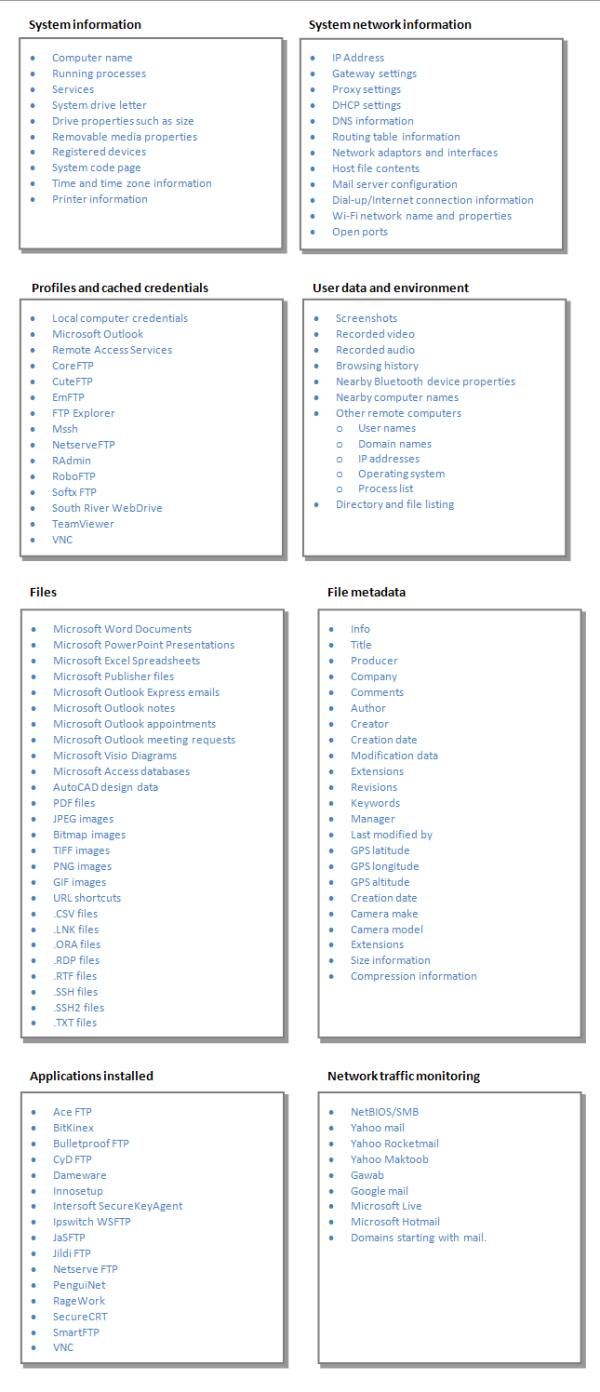
\includegraphics[width=6.00cm]{img/685331.jpg}
	~\\ \emph{L'ensemble des donn{\'e}es r{\'e}colt{\'e}es par Flame, selon Symantec.}
\end{minipage}
~\footnotetext{\texttt{http://www.symantec.com/connect/blogs/w32flamer-enormous-data-collection}}

Cette infection sournoise a aussi n{\'e}cessit{\'e} l'utilisation d{\'e}tourn{\'e}e de certificats pourtant sign{\'e}s par Microsoft afin que le logiciel s'installe sans la moindre alerte. La firme de Redmond a, depuis, \texttt{r{\'e}voqu{\'e} les certificats en question~\footnote{\texttt{http://blogs.technet.com/b/srd/archive/2012/06/03/microsoft-certification-authority-signing-certificates-added-to-the-untrusted-certificate-store.aspx}}} et propose une mise {\`a} jour de s{\'e}curit{\'e} sur... Windows Update, {\'e}videmment !~\\

\begin{minipage}[ht]{6.25cm}	
	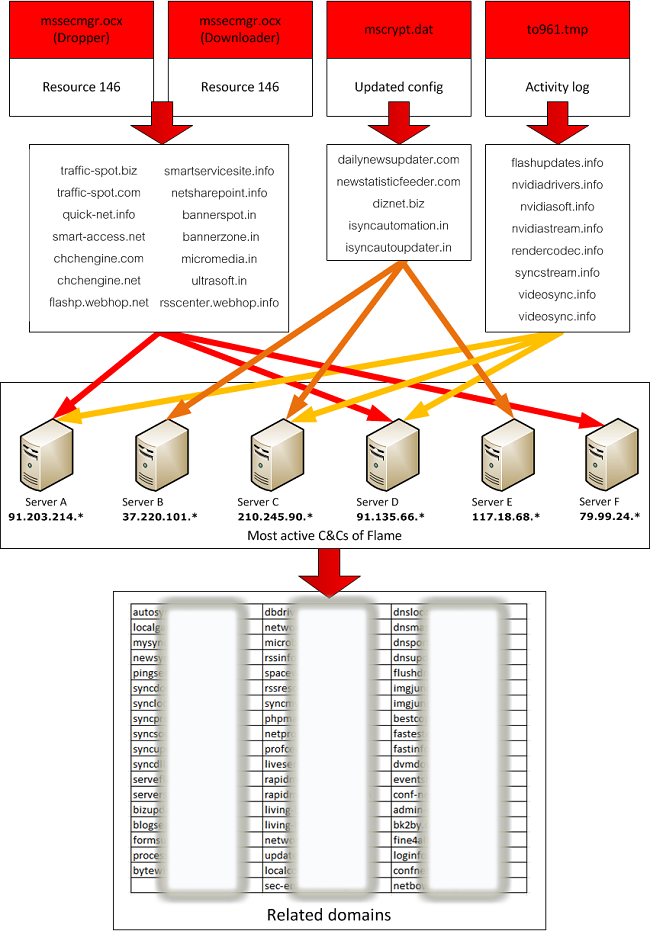
\includegraphics[width=6.00cm]{img/685335.png}
	~\\ \emph{La structure de contr{\^o}le et de commande de Flame, selon Kaspersky.}
\end{minipage} \hfill \begin{minipage}[ht]{12.50cm}
	\small
	\textbf{\large Une arme en fonction au moins depuis 2008}~\\
	
	Kaspersky a par ailleurs publi{\'e} une \texttt{longue analyse de la structure de contr{\^o}le et de commande de Flame~\footnotemark }, qui permet {\`a} ses op{\'e}rateurs de piloter leur b{\'e}b{\'e} {\`a} distance et de r{\'e}cup{\'e}rer les informations r{\'e}colt{\'e}es. L'entreprise s'est pour cela associ{\'e}e {\`a} la firme GoDaddy (o{\`u} {\'e}taient enregistr{\'e}s la plupart des domaines) et {\`a} OpenDNS, afin de d{\'e}tourner les domaines sur leur propre << \emph{sinkhole} >> et ainsi tenter d'en savoir plus.~\\
	
	Et l{\`a} encore, les chiffres parlent d'eux-m{\^e}mes : la firme de s{\'e}curit{\'e} russe a trouv{\'e} pas moins de 80 noms de domaines li{\'e}s {\`a} l'infrastructure. Des noms {\'e}videmment enregistr{\'e}s avec une kyrielle de fausses identit{\'e}s et d'adresses bidons << \emph{en Allemagne et en Autriche, notamment {\`a} Vienne} >>. Il est par ailleurs int{\'e}ressant de noter que les premiers noms de domaine li{\'e}s {\`a} Flame ont {\'e}t{\'e} enregistr{\'e}s d{\`e}s 2008, ce qui prouve que la cyberarme est en fonction depuis bien longtemps ! Quant aux machines infect{\'e}es, si elles se situent essentiellement au Moyen-Orient, on en trouve aussi une dizaine aux Etats-Unis et quelques-unes en Europe... mais aucune en France pour le moment, d'apr{\`e}s les {\'e}tudes -- forc{\'e}ment partielles -- de Kaspersky.~\\
	
	Les op{\'e}rateurs de Flame ont en tout cas {\'e}t{\'e} des plus prudents : d'apr{\`e}s Symantec, d{\`e}s que le kit a {\'e}t{\'e} d{\'e}couvert, ils ont envoy{\'e} une commande d'autodestruction {\`a} certaines machines infect{\'e}es, sous la forme d'un nouveau fichier de << d{\'e}sinstallation >> qui a supprim{\'e} toute trace de leur \oe uvre.~\\
\end{minipage}
~\footnotetext{\texttt{http://www.securelist.com/en/blog/208193540/The\_Roof\_Is\_on\_Fire\_Tackling\_Flames\_C\_C\_Servers}}

\dotfill

\textbf{\large Flame, le premier malware Windows qui profite de Bluetooth}~\\

\begin{minipage}[ht]{6.25cm}
	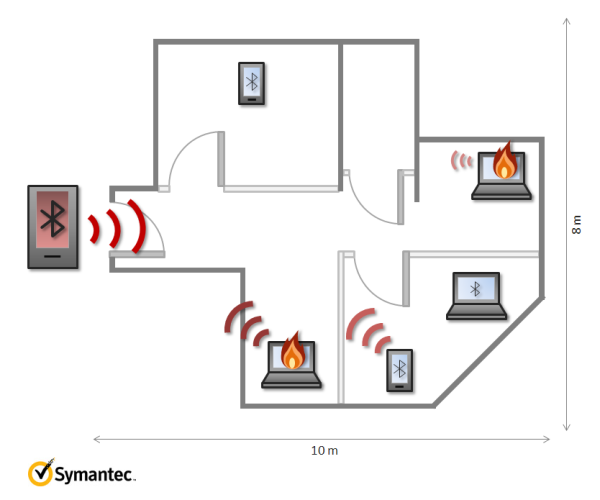
\includegraphics[width=6.00cm]{img/685339.png}
\end{minipage} \hfill \begin{minipage}[ht]{12.50cm}
	\small 
	C'est sans doute l'une des fonctions les plus incroyables de Flame : le kit d'espionnage est capable d'effectuer un rep{\'e}rage des appareils Bluetooth pr{\'e}sents autour de la machine infect{\'e}e. D'autre part, il transforme l'ordinateur en << balise >> Bluetooth, qui sera du coup rep{\'e}r{\'e}e par tous les autres appareils dans la zone.~\\
	
	Flame est, selon Symantec~\footnotemark, le seul code malveillant sous Windows {\`a} disposer d'une telle fonction. A quoi cela sert-il ? Le myst{\`e}re demeure. Mais la firme de s{\'e}curit{\'e} {\'e}labore des sc{\'e}narios probables, qui t{\'e}moigneraient encore du talent des d{\'e}veloppeurs.~\\
	
	L'utilisation du Bluetooth pourrait d'abord {\^e}tre la premi{\`e}re {\'e}tape d'une attaque qui n'a pas encore {\'e}t{\'e} d{\'e}couverte dans Flame : espionner un kit mains-libres, par exemple... ou exfiltrer des donn{\'e}es vol{\'e}es via Bluetooth par une connexion data d'un mobile, ce qui pourrait avoir comme avantage d'outrepasser des \emph{firewalls}...~\\
\end{minipage}
~\footnotetext{\texttt{http://www.symantec.com/connect/blogs/flamer-recipe-bluetoothache}}

Autre sc{\'e}nario possible : Flame pourrait profiter des informations r{\'e}colt{\'e}es pour en savoir plus sur les connaissances de la victime. << \emph{Alors que, le temps passant, la victime rencontre des amis et des associ{\'e}s, les attaquants pourraient cataloguer les diff{\'e}rents appareils qu'elle ``rep{\`e}re'', notamment des t{\'e}l{\'e}phones mobiles. De cette mani{\`e}re, les attaquants pourraient {\'e}tablir une carte des interactions avec diverses personnes et identifier les cercles personnels et professionnels de la victime. } >>~\\

Encore plus fort, Symantec imagine un sc{\'e}nario dans lequel cette utilisation du Bluetooth servirait {\`a} traquer la position de la victime : << \emph{en mesurant la puissance d'une onde radio, un attaquant pourrait mesurer si la victime s'approche ou s'{\'e}loigne d'un appareil particulier} >>. L'entreprise va jusqu'{\`a} {\'e}voquer une intrigue {\`a} la James Bond, dans laquelle la victime pourrait {\^e}tre suivie {\`a} la trace par de puissants appareils de surveillance Bluetooth dans les a{\'e}roports, gares etc. Simplement en s'appuyant sur l'adresse Bluetooth de son t{\'e}l{\'e}phone portable, pr{\'e}alablement r{\'e}colt{\'e}e par Flame.~\\

<< \emph{Ces th{\'e}ories sont faciles {\`a} impl{\'e}menter pour un attaquant talentueux. La sophistication de W32.Flamer indique que ses cr{\'e}ateurs sont certainement habiles techniquement et ces attaques sont parfaitement {\`a} leur port{\'e}e} >>, conclut Symantec.~\\


\clearpage

\texttt{http://www.lemonde.fr/technologies/article/2012/05/29/decouverte-d-un-nouveau-programme-malveillant-flame\_1708752\_651865.html}

\textbf{\LARGE D{\'e}couverte d'un nouveau programme malveillant : Flame}~\\

\textbf{\small Le Monde.fr | 29.05.2012 {\`a} 10h40}~\\

\begin{minipage}[ht]{6.25cm}
	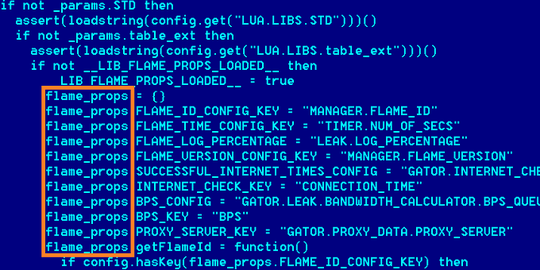
\includegraphics[width=6.00cm]{img/1708759_3_0e13_le-code-du-systeme-d-information-flame_37d6fd3dbe7b7274419e2accf220835e.png}
	~\\ \emph{\small Le code du syst{\`e}me d'information Flame.}
\end{minipage} \hfill \begin{minipage}[ht]{12.50cm}
	\small 
	L'{\'e}diteur de solutions antivirus Kaspersky a annonc{\'e}, lundi 28 mai, avoir d{\'e}couvert un nouveau programme malveillant, qui a infect{\'e}~\footnotemark un grand nombre d'ordinateurs en Iran et dans la r{\'e}gion isra{\'e}lo-palestinienne, avant le Soudan et la Syrie. L'attaque aurait vis{\'e} des repr{\'e}sentants {\'e}tatiques, mais aussi des universitaires, selon les {\'e}tudes pr{\'e}liminaires.~\\
	
	Baptis{\'e} Flame, le programme serait "\emph{dans la nature depuis au moins deux ans. Mais {\`a} cause de son extr{\^e}me complexit{\'e}, aucun logiciel de s{\'e}curit{\'e} n'a pu le d{\'e}tecter}", indique Kaspersky. A la diff{\'e}rence de Stuxnet, ou m{\^e}me de Duqu, un autre virus capable de collecter des informations, "\emph{l'objectif premier de Flame est le cyberespionnage et le vol d'informations pr{\'e}sentes sur les machines infect{\'e}es}".~\\
\end{minipage}
~\footnotetext{\texttt{http://www.wired.com/threatlevel/2012/05/flame/}}

"\emph{C'est une porte d{\'e}rob{\'e}e, un cheval de Troie, mais aussi un programme dot{\'e} de fonctionnalit{\'e}s proches d'un ver informatique}", explique le site Secure List. Une fois qu'il infecte un ordinateur, Flame obtient diverses sortes de donn{\'e}es stock{\'e}es sur l'appareil, est capable de prendre des photographies,  d'enregistrer des conversations audio et de reconna{\^i}tre les mots de passe tap{\'e}s par l'utilisateur.~\\

Le mode d'infection demeure toutefois inconnu. "\emph{Nous avons des suspicions {\`a} propos de l'exploitation d'une vuln{\'e}rabilit{\'e} de Windows, mais nous ne pouvons pas encore le confirmer}", note Secure List. L'origine de l'attaque fait {\'e}galement l'objet de sp{\'e}culations, mais selon les experts, cit{\'e}s par le \emph{Washington Post~\footnote{\texttt{http://www.washingtonpost.com/world/national-security/newly-identified-computer-virus-used-for-spying-is-20-times-size-of-stuxnet/2012/05/28/gJQAWa3VxU\_story.html\%20Secure\%20list\%20https://www.securelist.com/en/blog?SSL=1\#}}}, la sophistication du programme laisse penser qu'une puissance {\'e}tatique a particip{\'e} {\`a} son {\'e}laboration. Mais comme l'indique Secure List, "\emph{il n'y a aucune information dans le code, qui permette d'identifier une quelconque nation. Donc, comme pour Stuxnet et Duqu, les auteurs demeurent inconnus}".~\\

Apr{\`e}s les annonces de Kaspersky, les autorit{\'e}s iraniennes ont annonc{\'e} avoir d{\'e}velopp{\'e} un outil permettant de suppimer ce nouveau programme malveillant.~\\

\texttt{http://www.lemonde.fr/technologies/article/2012/06/11/le-virus-informatique-flame-a-disparu\_1716050\_651865.html}~\\

\textbf{\LARGE Le virus informatique Flame a disparu}~\\

\textbf{\small Le Monde.fr avec AFP | 11.06.2012 {\`a} 07h26 -- Mis {\`a} jour le 11.06.2012 {\`a} 09h57}~\\

Le virus informatique Flame, d{\'e}tect{\'e} r{\'e}cemment et qualifi{\'e} de "\emph{cyberarme}", qui visait notamment {\`a} d{\'e}rober des documents li{\'e}s au programme nucl{\'e}aire iranien, a re\c{c}u l'ordre de dispara{\^i}tre sans laisser de trace, selon la soci{\'e}t{\'e} de s{\'e}curit{\'e} informatique Symantec. --- "\emph{A la fin de la semaine derni{\`e}re, certains centres de commande de Flame ont envoy{\'e} un nouvel ordre {\`a} plusieurs ordinateurs contamin{\'e}s, a indiqu{\'e} dimanche \texttt{Symantec~\footnote{\texttt{http://www.symantec.com/connect/blogs/flamer-urgent-suicide}}} sur son blog. Cet ordre est destin{\'e} {\`a} faire compl{\`e}tement dispara{\^i}tre Flame des ordinateurs compromis.}"~\\

Le virus Flame a {\'e}t{\'e} d{\'e}tect{\'e} dans diff{\'e}rentes r{\'e}gions du monde, notamment au Moyen-Orient, en Europe, en Am{\'e}rique du Nord et en Asie-Pacifique, l'Iran {\'e}tant le premier pays vis{\'e} par ces attaques.~\\

Le virus existait depuis quatre ans, mais il n'avait {\'e}t{\'e} identifi{\'e} qu'{\`a} la fin de mai par le fabricant russe d'antivirus Kaspersky Lab, qui avait not{\'e} que la sophistication de ce virus utilis{\'e} {\`a} des fins de "\emph{cyberespionnage}" {\'e}tait telle qu'il supposait le concours d'un Etat.~\\

Apr{\`e}s cette annonce, le ministre des affaires strat{\'e}giques isra{\'e}lien Mosh{\'e} Yaalon avait justifi{\'e} le recours {\`a} de tels virus afin de contrer la menace nucl{\'e}aire iranienne. %% ~\\

\clearpage

\texttt{https://korben.info/quand-les-enfants-jouent-avec-des-armes-quils-ne-maitrisent-pas.html}~\\

\textbf{\LARGE Quand les enfants jouent avec des armes qu'ils ne maitrisent pas...}~\\

par Korben~\\


\includegraphics[width=0.80\textwidth]{img/capture05072008115135bm6.jpg}

Donc, voil{\`a}, c'est confirm{\'e} ! Le virus \texttt{Stuxnet~\footnote{\texttt{http://en.wikipedia.org/wiki/Stuxnet}}} est bien co-cr{\'e}ation diabolique mise au point par les {\'E}tats-Unis et Isra{\"e}l. Ce n'est pas moi qui le dit mais une longue enqu{\^e}te en profondeur du \texttt{New York Times~\footnote{\texttt{http://www.nytimes.com/2012/06/01/world/middleeast/obama-ordered-wave-of-cyberattacks-against-iran.html?pagewanted=all}}}. Le code de Stuxnet {\'e}tait suppos{\'e} au d{\'e}part n'infecter que les installations iraniennes afin de contrer les ambitions nucl{\'e}aires du pays, mais bizarrement, la bestiole a {\'e}chapp{\'e} {\`a} ses cr{\'e}ateurs.~\\

Le projet Stuxnet, lanc{\'e} sous la pr{\'e}sidence de George W. Bush avait l'avantage de permettre au gouvernement am{\'e}ricain d'atteindre le c\oe ur du r{\'e}seau gouvernemental iranien situ{\'e} {\`a} \texttt{Natanz~\footnote{\texttt{http://maps.google.com/maps?ll=33.5133333333,51.9163888889\&spn=0.1,0.1\&q=33.5133333333,51.9163888889\%20\%28Natanz\%29\&t=h}}}, non accessible depuis l'ext{\'e}rieur...Implant{\'e} sur place par un agent double (en tout cas, c'est l'hypoth{\`e}se la plus probable), le virus s'est {\'e}videmment {\'e}chapp{\'e} vers le r{\'e}seau public gr{\^a}ce au "facteur humain" qui trimballe toujours tout un tas de trucs sur cl{\'e} USB... Ainsi, le virus a pu {\^e}tre transport{\'e} {\`a} l'insu des Iraniens, du r{\'e}seau de Natanz vers le r{\'e}seau Internet grand public.~\\

Oups !~\\

Selon les am{\'e}ricains, Stuxnet n'aurait jamais d{\^u} pouvoir se propager {\`a} l'ext{\'e}rieur, mais toujours d'apr{\`e}s eux, les Isra{\'e}liens ont fait des modifs dans Stuxnet {\`a} leur insu, rendant la propagation possible...~\\

C'est quand m{\^e}me con.. Mais c'est ce qui arrive avec les armes. Car oui, Stuxnet est une arme dont les Am{\'e}ricains et les isra{\'e}liens ont perdu le contr{\^o}le et qui s'est retourn{\'e}e contre toutes les nations du monde entier. Heureusement, les d{\'e}g{\^a}ts sont rest{\'e}s "techniques" et aucune vie humaine n'a subi de cons{\'e}quences directes {\`a} cause de Stuxnet mais si ce dernier avait pour but par exemple de d{\'e}clencher l'explosion de centrales nucl{\'e}aires ou de missiles directement dans leurs silos ou de faire s'{\'e}craser des satellites, voir des avions, je pense que nous aurions tous beaucoup moins rigol{\'e}.~\\

Bref, les {\'E}tats-Unis nous ont donn{\'e} un parfait exemple ici que maintenant la guerre c'est dans le cyber-espace, m{\^e}me en temps de "paix" et que malheureusement, mal maitris{\'e}es, ces technologies peuvent vite foutre un bordel mondial.~\\

Que se passera-t-il {\`a} la prochaine boulette ? Sachant que les {\'E}tats-Unis ont d{\'e}clar{\'e} que \texttt{tout acte de guerre d{\'e}clench{\'e}e dans le cyber-espace pourrait avoir une r{\'e}ponse militaire~\footnote{\texttt{http://www.telegraph.co.uk/news/worldnews/northamerica/usa/8550642/US-could-respond-to-cyber-attack-with-conventional-weapons.html}}} dans le monde r{\'e}el, on se demande ce que \c{c}a aurait donn{\'e} si Stuxnet avait {\'e}t{\'e} un produit Iranien, Chinois, Russe, voire m{\^e}me Europ{\'e}en...~\\

Brrrr.... --- Reste {\`a} savoir maintenant qui est le papa de \texttt{Flame~\footnote{\texttt{http://www.cbsnews.com/8301-501465\_162-57443071-501465/flame-computer-virus-strikes-middle-east-israel-speculation-continues/}}}... :-)~\\

\texttt{Source~\footnote{\texttt{http://arstechnica.com/tech-policy/2012/06/confirmed-us-israel-created-stuxnet-lost-control-of-it/}}}~\\

\clearpage

\texttt{http://www.journaldugeek.com/2012/03/09/trojan-duqu-kaspersky-demande-de-laide/}~\\

\textbf{\LARGE Trojan Duqu : Kaspersky demande de l'aide}~\\

\textbf{\small Par Chrystelle, 09 mars 2012 {\`a} 11:55}~\\

\begin{minipage}[ht]{6.25cm}
	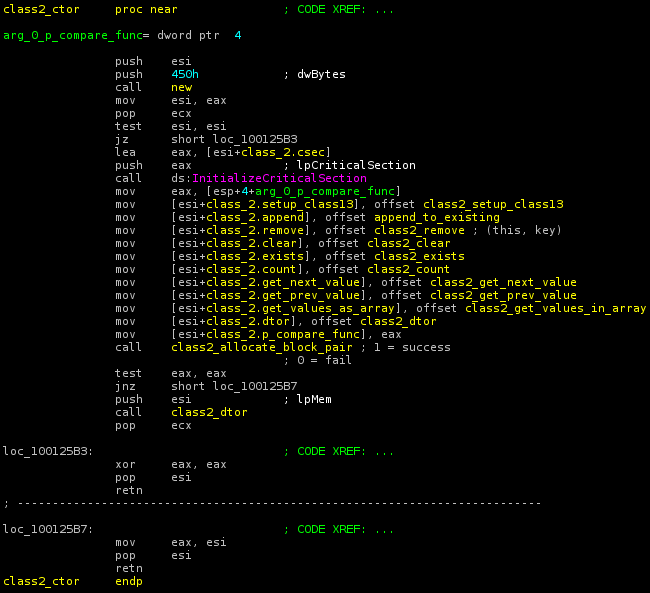
\includegraphics[width=6.00cm]{img/Duqu.png}
\end{minipage} \hfill \begin{minipage}[ht]{12.50cm}
	\small
	Duqu est un trojan qui a pour but de s'infiltrer dans le syst{\`e}me afin de voler des informations priv{\'e}es. Ce trojan touche plus particuli{\`e}rement l'Iran et a pour cible les centrales nucl{\'e}aires iraniennes. \textbf{Ce dernier donne du fil {\`a} retordre aux experts de la c{\'e}l{\`e}bre soci{\'e}t{\'e} Kaspersky qui est sp{\'e}cialis{\'e}e dans la s{\'e}curit{\'e} des syst{\`e}mes d'information, car m{\^e}me si une grande partie du programme a {\'e}t{\'e} d{\'e}velopp{\'e}e en C++, il semblerait qu'une partie du langage soit encore inconnue des ing{\'e}nieurs. }~\\

	\textbf{\large Une demande d'aide par Kaspersky}~\\

	A part quelques r{\'e}f{\'e}rences {\`a} Stuxnet 2.0 (un ver con\c{c}u pour attaquer une cible industrielle), Duqu reste un myst{\`e}re en ce qui concerne le langage utilis{\'e} pour la prise en charge des communications. Un ing{\'e}nieur de chez Kaspersky a donc demand{\'e} de l'aide aupr{\`e}s des internautes sur son blog. Pour le moment, une seule {\'e}bauche a {\'e}t{\'e} donn{\'e}e par un internaute, indiquant que ce langage << inconnu >> pourrait provenir de compilateurs IBM pour les vieux mainframe (ordinateur central de grande puissance) OS400 SYS38/SYS36.~\\	
\end{minipage}	

\textbf{Les principales conclusions donn{\'e}es :}
\begin{itemize}
	\small
	\item Le Framework de Duqu a {\'e}t{\'e} {\'e}crit dans un langage de programmation inconnu.
	\item Contrairement  au corps du programme, le reste du langage de programmation de Duqu n'est pas en C++ et n'a pas {\'e}t{\'e} compil{\'e} avec Microsoft Visual C++.
	\item L'architecture du code a {\'e}t{\'e} con\c{c}ue pour {\^e}tre utilis{\'e}e dans n'importe quel type de conditions, incluant des commutations asynchrones.
	\item Si on se r{\'e}f{\`e}re {\`a} la taille du projet Duqu, il est fort probable que l'{\'e}quipe qui se soit charg{\'e}e du Framework ne soit pas la m{\^e}me que celle {\`a} l'origine des pilotes et de l'{\'e}criture de l'infection du syst{\`e}me.
	\item Ce myst{\'e}rieux langage de programmation n'est d{\'e}finitivement pas du C++, Objective C, Java, Python, Ada, Lya et autres langages connus.
\end{itemize}

\texttt{Source~\footnote{\texttt{http://www.theinquirer.net/inquirer/news/2158090/kaspersky-claims-duqu-trojan-programming-language}}}~\\

%% \clearpage

\texttt{http://www.theinquirer.net/inquirer/news/2158090/kaspersky-claims-duqu-trojan-programming-language}~\\

\textbf{\LARGE Kaspersky claims Duqu Trojan uses its own programming language}~\\

Complexity further suggests state involvement~\\

\textbf{\small By Lawrence Latif -- The Inquirer -- Thu Mar 08 2012, 13:30}~\\

\textbf{SECURITY OUTFIT} Kaspersky Lab claims that part of the Duqu Trojan was written in a bespoke programming language.~\\

Kaspersky claims that unlike the rest of the Duqu Trojan, which is written in C++, part of the code in the payload dynamic linked library is made up of a yet unidentified programming language. According to Kaspersky the language is not C++ and was not compiled with Microsoft's Visual C++, however it is an object-oriented programming language.~\\

Kaspersky confirms the language has "related activities that are suitable for network applications", meaning that it has some level of access to a network adaptor, though the firm didn't say what sort of low-level access. The Duqu Trojan uses command and control servers on the internet to operate, meaning that some level of network connectivity is a must.~\\

\clearpage %% !!

Alexander Gostev, chief security expert at Kaspersky Lab said, "With the extremely high level of customisation and exclusivity that the programming language was created with, it is also possible that it was made not only to prevent external parties from understanding the cyber-espionage operation and the interactions with the C and Cs [command and control servers], but also to keep it separate from other internal Duqu teams who were responsible for writing the additional parts of the malicious program."~\\

While Kaspersky was unable to identify the programming language used, it shows that the programmers went to great lengths to create an object-oriented programming language and an associated compiler for the Duqu Trojan. Given the apparent complexity of such a task, this gives further credence to claims that the Duqu Trojan, which has mainly affected Iranian systems, was designed and written by more than just some lone cheeky chap looking to cause random disruption. %% ~\\

\rule{\textwidth}{0.01cm} %% \clearpage

\texttt{http://www.journaldugeek.com/2012/03/22/kaspersky-a-eu-duqu/}~\\

\textbf{\LARGE Kaspersky a eu DuQu}~\\

\textbf{\small Par Chrystelle, 22 mars 2012 {\`a} 14:33}~\\

\begin{minipage}[ht]{6.25cm}
	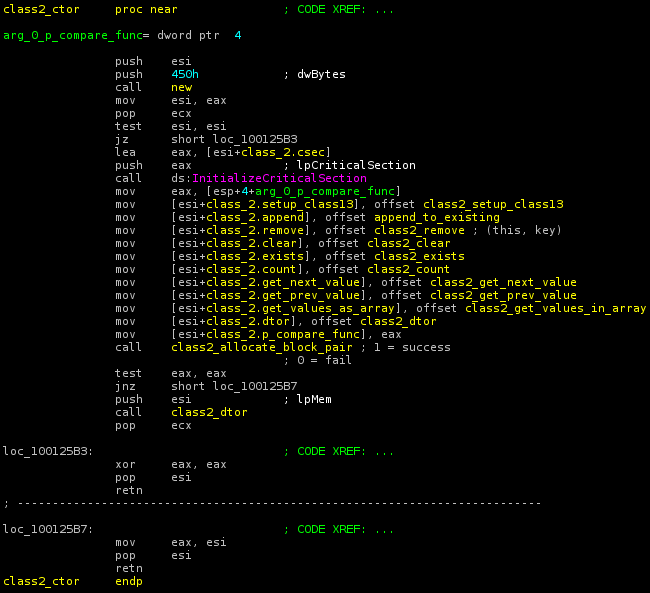
\includegraphics[width=6.00cm]{img/Duqu.png}
\end{minipage} \hfill \begin{minipage}[ht]{12.50cm}
	\small
	Des nouvelles du trojan DuQu, qui donnait du fil {\`a} retordre aux experts de chez Kaspersky, dont le langage utilis{\'e} restait un myst{\`e}re pour le laboratoire. Kaspersky avait demand{\'e} de l'aide {\`a} la communaut{\'e}~\footnotemark et re\c{c}u de nombreuses r{\'e}ponses. Il semblerait donc que le langage utilis{\'e} ne soit pas si inconnu que \c{c}a, puisqu'il a {\'e}t{\'e} {\'e}crit en C, orient{\'e} objet (OO C) gr{\^a}ce {\`a} un framework personnalis{\'e}, le tout compil{\'e} avec Microsoft Visual Studio Compiler 2008. La technique, si je puis dire, {\`a} l'ancienne.~\\
	
	\textbf{Conclusion d'Igor Soumenkov de Kapersky Labs :}

	\emph{Nos conclusions indiquent une {\'e}quipe de d{\'e}veloppeurs professionnels qui r{\'e}utilisent du vieux code [...] A l'heure actuelle, ces techniques sont plus g{\'e}n{\'e}ralement utilis{\'e}es pour la cr{\'e}ation de logiciels professionnels plut{\^o}t que pour la cr{\'e}ation de logiciels malveillants. Une nouvelle fois, tout indique que DuQu, tout comme Stuxnet, est un malware unique en son genre, qui se dresse comme une gemme se distinguant du grand nombre de programmes malveillants que nous avons g{\'e}n{\'e}ralement l'habitude de voir.}~\\
\end{minipage}~\\
~\footnotetext{\texttt{http://www.journaldugeek.com/2012/03/09/trojan-duqu-kaspersky-demande-de-laide/}}


\texttt{Source~\footnote{\texttt{http://thehackernews.com/2012/03/mystery-of-duqu-programming-language.html}}}

\clearpage

\texttt{http://thehackernews.com/2012/03/mystery-of-duqu-programming-language.html}~\\



\textbf{\LARGE Mystery of Duqu Programming Language Solved}~\\

\textbf{\small Posted On 3/20/2012 07:09:00 AM By THN Security Analyst}~\\

\begin{minipage}[ht]{6.25cm}
	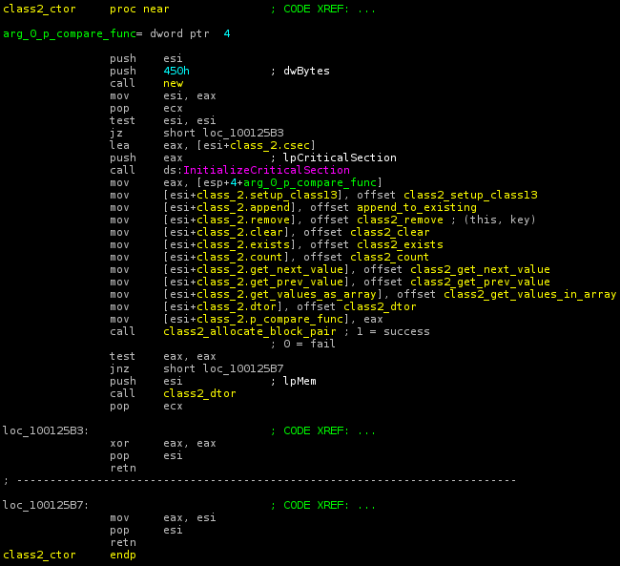
\includegraphics[width=6.00cm]{img/MysteryOfDuquProgrammingLanguageSolved.png}
\end{minipage} \hfill \begin{minipage}[ht]{12.50cm}
	\small
	An \texttt{appeal for help~\footnotemark} from the programming community has allowed antivirus analysts to classify the unknown language used to develop key components of the Duqu Trojan. The sections responsible for downloading and executing additional modules in the Duqu Trojan, referred to by some as Stuxnet 2.0, were written in standard C++.~\\

	Kaspersky Lab experts now say with a high degree of certainty that the Duqu framework was written using a custom object-oriented extension to C, generally called ``OO C'' and compiled with Microsoft Visual Studio Compiler 2008 (MSVC 2008) with special options for optimizing code size and inline expansion.~\\
\end{minipage}~\\
~\footnotetext{\texttt{http://thehackernews.com/2012/03/duqu-trojan-developed-in-unknown.html}}

Kaspersky's Igor Soumenkov wrote, ``\emph{No matter which of these two variants is true, the implications are impressive. The Payload DLL contains 95 Kbytes of event-driven code written with OO C, a language that has no automatic memory management or safe pointers. }''.~\\

\textbf{Kaspersky's analysis now concludes:}
\begin{itemize}
	\item The Duqu Framework consists of ``C'' code compiled with MSVC 2008 using the special options ``/O1'' and ``/Ob1''
	\item The code was most likely written with a custom extension to C, generally called ``OO C''
	\item The event-driven architecture was developed as a part of the Duqu Framework or its OO C extension
	\item The C\&C code could have been reused from an already existing software project and integrated into the Duqu Trojan
\end{itemize}~\\

The Duqu Framework may have been created by a different programming team, since it is unique to Duqu, unlike many parts of Duqu that seem to be directly borrowed from Stuxnet. It's believed that the developers are old school that don't trust C++ and that's probably why they relied on C. Another reason for using OO C is because back in the good old days it was more portable than C++.~\\ 

Knowing the techniques used to develop the malware allows Kaspersky's researchers to make better guesses about who might be behind the code. Creating Duqu was a major project, so it's possible that an entirely different team was responsible for creating the Duqu Framework, while others worked on creating drivers and system infection exploits. In this scenario it's even possible that those who created the Duqu framework were ignorant of the real purpose of their work.~\\

Duqu was first detected in September 2011, but Kaspersky Lab believes it has seen the first pieces of Duqu-related malware dating back to August 2007. The Russian security firm also notes Duqu, like Stuxnet before it, is highly targeted and related to Iran's nuclear program.~\\

\clearpage

\texttt{http://www.linformaticien.com/actualites/id/24104/malware-duqu-du-travail-de-pros.aspx}~\\

\textbf{\LARGE Malware Duqu : du travail de pros}~\\

\textbf{\small par St{\'e}phane Larcher, le 20 mars 2012 16:16}~\\

\textbf{On s'en doutait mais Kaspersky Labs aid{\'e} par la communaut{\'e} de programmeurs le confirme : Le malware Duqu, lui-m{\^e}me inspir{\'e} de Stuxnet, n'a pas {\'e}t{\'e} con\c{c}u par des "petits jeunes qui d{\'e}butent" mais par des vrais pros du d{\'e}veloppement. }~\\

C'est dans les vieux pots qu'on fait les meilleures soupes. La jeune g{\'e}n{\'e}ration de programmeurs serait bien avis{\'e}e de s'inspirer de cet adage car l'analyse faite par une communaut{\'e} de programmeurs venus {\`a} l'aide de Kaspersky montre que le langage C, le vieux --  l'unique pour certains -- a {\'e}t{\'e} employ{\'e} pour concevoir Duqu et Stuxnet. Et ceci n'est pas forc{\'e}ment une bonne nouvelle.~\\

Revenons sur la gen{\`e}se de cette d{\'e}couverte. Depuis de nombreux mois les analystes et experts de l'{\'e}diteur russe Kaspersky Labs plongent dans les entrailles de Duqu. Et d'ores et d{\'e}j{\`a} ils {\'e}taient arriv{\'e}s {\`a} des conclusions un peu inqui{\'e}tantes {\`a} savoir que Duqu et Stuxnet avaient {\'e}t{\'e} cr{\'e}{\'e}s {\`a} partir d'une m{\^e}me plate-forme datant de fin 2007, d{\'e}but 2008 et modifi{\'e}e en 2010 pour concevoir les deux malwares sus-nomm{\'e}s. Le probl{\`e}me vient du fait que cette "plate-forme" a conduit {\`a} la la cr{\'e}ation et la d{\'e}couverte de Stuxnet et Duqu mais rien n'indique qu'il n'y en a pas d'autres dans la nature. Et plus exactement, la probabilit{\'e} la plus forte est qu'il en existe de nouveaux qui -eux -- n'ont pas encore {\'e}t{\'e} d{\'e}couverts.~\\
Jusqu'ici, les chercheurs de Kaspersky butaient encore sur une partie de code de Duqu dont ils ne parvenaient pas {\`a} imaginer le langage de d{\'e}part. Ils avaient donc fait appel {\`a} la communaut{\'e} de programmeurs pour les aider dans leurs recherches. Kaspersky indique avoir re\c{c}u une quantit{\'e} incroyable de pr{\'e}cieux commentaires et que certains d'entre eux leur permettent aujourd'hui d'affirmer que le Framework de Duqu (la partie qui permet de communiquer avec les serveurs de commande et de contr{\^o}le du Cheval de Troie une fois que celui-ci a infect{\'e} la machine) est {\'e}crit en C. Il est ensuite compil{\'e} avec Visual Studio 2008 avec des options sp{\'e}ciales pour optimiser la taille du code et son expansion en ligne. De fait le code g{\'e}n{\'e}r{\'e} est ce que l'on appelle du OO C pour Object Oriented C. Bref, il ne s'agit pas de C++ mais de bon vieux C int{\'e}grant une composante objet. Et une nouvelle fois, le fait que les concepteurs de ces virus aient employ{\'e} du C plut{\^o}t  que du C++ ne constitue pas non plus une excellente nouvelle.~\\

\textbf{\large Des programmeurs chevronn{\'e}s}~\\

En effet, Les programmeurs de la vieille {\'e}cole -- les purs, les durs, les tatou{\'e}s -- ont toujours exprim{\'e} des r{\'e}serves par rapport au C++, consid{\'e}rant que les m{\'e}thodes d'allocation de la m{\'e}moire n'{\'e}taient pas satisfaisantes et d{\'e}non\c{c}ant des fonctions obscures risquant de causer indirectement l'ex{\'e}cution de code. "\emph{le C et accessoirement l'OO C fournirait un cadre plus faible, moins propice aux comportements impr{\'e}vus}", indique Kaspersky dans un communiqu{\'e}. La seconde raison est la portabilit{\'e}. A ses d{\'e}buts, le C++ n'{\'e}tait pas aussi normalis{\'e} qu'il l'est aujourd'hui et le code n'{\'e}tait donc pas compatible avec tous les compilateurs. Le C, a contrario, se caract{\'e}rise par une portabilit{\'e} extr{\^e}me. La conclusion d'Igor Soumenkov, expert au sein de Kaspersky Labs est la suivante :~\\
"\emph{Ces deux raisons donnent {\`a} penser que le code a {\'e}t{\'e} {\'e}crit par une {\'e}quipe de d{\'e}veloppeurs chevronn{\'e}s <<de la vieille {\'e}cole>>, souhaitant cr{\'e}er une plate-forme personnalis{\'e}e pour le lancement d'une attaque d'une grande souplesse et adaptabilit{\'e}. Ce code pourrait avoir {\'e}t{\'e} repris de pr{\'e}c{\'e}dentes cyberattaques et adapt{\'e} de fa\c{c}on {\`a} s'int{\'e}grer au cheval de Troie Duqu. Cependant, une chose est s{\^u}re : ces techniques sont normalement l'apanage de programmeurs d'{\'e}lite et ne se rencontrent aujourd'hui quasiment jamais dans les malwares en g{\'e}n{\'e}ral. } " %% ~\\

\clearpage

\texttt{http://www.linformaticien.com/actualites/id/24470/stuxnet-un-agent-double-aurait-accelere-l-infection.aspx}~\\

\textbf{\LARGE Stuxnet : un agent double aurait acc{\'e}l{\'e}r{\'e} l'infection}~\\

\textbf{\small par St{\'e}phane Larcher, le 13 avril 2012 15:06}~\\

\textbf{Le site ISS Source r{\'e}v{\`e}le de nouvelles informations concernant Stuxnet. L'attaque aurait {\'e}t{\'e} men{\'e}e par un dissident iranien infiltr{\'e} dans la centrale de Natanz qui se serait charg{\'e} du sabotage {\`a} l'aide d'une barrette m{\'e}moire infect{\'e}e.}~\\

On commence enfin {\`a} en savoir un peu plus sur la mani{\`e}re dont s'est d{\'e}roul{\'e}e l'attaque Stuxnet visant les installations nucl{\'e}aires en Iran et dont on a d{\'e}couvert l'existence au mois de juin 2010 par le biais de la soci{\'e}t{\'e} bi{\'e}lorusse VirusBlokAda.~\\

ISS Source indique qu'outre les techniques d'infection distantes possibles, le virus aurait {\'e}t{\'e} inject{\'e} directement dans une centrale nucl{\'e}aire par un agent double iranien intervenant dans la centrale nucl{\'e}aire de Natanz. Cette injection directe, par le biais d'une barrette m{\'e}moire contenant le virus, pr{\'e}sentait l'int{\'e}r{\^e}t d'accro{\^i}tre consid{\'e}rablement les possibilit{\'e}s d'infection d'un grand nombre d'ordinateurs. Finalement, il semble que 45 000 syst{\`e}mes informatiques aient {\'e}t{\'e} infect{\'e}s, dont 30 000 en Iran.~\\

Notons que cette hypoth{\`e}se se r{\'e}v{\`e}le conforme {\`a} ce qu'indiquait le ministre iranien Heydar Moslehi  en octobre 2010, affirmant que des espions avaient {\'e}t{\'e} arr{\^e}t{\'e}s en lien avec le virus Stuxnet.~\\

ISS Source pr{\'e}cise que ces agents doubles appartiendraient au Mujahedeen-e-khalq (MEK), une organisation utilis{\'e}e par Isra{\"e}l pour diff{\'e}rentes missions, notamment les assassinats cibl{\'e}s visant des scientifiques en charge du programme nucl{\'e}aire iranien. << \emph{Le MEK est le bras arm{\'e} du Mossad en charge des assassinats} >>, pr{\'e}cise Vince Cannistraro, en charge du contre-terrorisme {\`a} la CIA. Ces agents seraient entra{\^i}n{\'e}s en Isra{\"e}l et ex{\'e}cuteraient les ordres fournis par l'{\'e}tat h{\'e}breu.~\\ 

\textbf{\large Nouveau sommet de la derni{\`e}re chance}~\\

Pour en revenir {\`a} Stuxnet, les autorit{\'e}s am{\'e}ricaines estiment que l'infection aurait commenc{\'e} d{\`e}s la mise en place de la barrette m{\'e}moire contenant le virus par le biais de l'une des trois failles Z{\'e}ro-day pr{\'e}sentes dans le virus. Ensuite, le virus se serait propag{\'e} {\`a} travers tout le r{\'e}seau en exploitant les autres failles tout en {\'e}tant per\c{c}u comme un programme << normal >> gr{\^a}ce {\`a} la pr{\'e}sence de certificats d{\'e}rob{\'e}s et embarqu{\'e}s au sein du << malware >>.~\\

Ces r{\'e}v{\'e}lations interviennent {\`a} la veille d'un nouveau sommet entre l'Iran d'un c{\^o}t{\'e} et le groupe 5+1 (Les cinq membres permanent du conseil de s{\'e}curit{\'e} de l'ONU + l'Allemagne) qui doit se d{\'e}rouler ce week-end {\`a} Istanbul. Ce sommet, une nouvelle fois pr{\'e}sent{\'e} comme le sommet de la derni{\`e}re chance, a pour objectif de trouver un accord sur la limitation du programme nucl{\'e}aire iranien. En effet, les tensions sont toujours plus vives et les isra{\'e}liens semblent d{\'e}termin{\'e}s {\`a} employer la force pour an{\'e}antir les installations nucl{\'e}aires d'Iran, une option militaire qui suscite de larges r{\'e}serves et inqui{\'e}tudes parmi les autres nations.~\\

\clearpage

\texttt{http://www.linformaticien.com/actualites/id/24986/flame-l-outil-de-cyberespionnage-le-plus-puissant-jamais-identifie.aspx}~\\

\textbf{\LARGE Flame : l'outil de cyberespionnage le plus puissant jamais identifi{\'e}}~\\

\textbf{\small par St{\'e}phane Larcher, le 29 mai 2012 13:42}~\\

\textbf{L'{\'e}diteur de s{\'e}curit{\'e} Kaspersky vient de publier ses premi{\`e}res conclusions concernant un malware d'un nouveau genre, d{\'e}crit comme le plus puissant et le plus complexe jamais identifi{\'e}. }~\\

Nous savons Kaspersky peu avare de superlatifs lorsqu'il s'agit de d{\'e}crire un malware. Mais la d{\'e}couverte de Flame d{\'e}passe tous les commentaires que l'on a pu entendre, y compris pour des virus comme Stuxnet ou Duqu. A l'instar de ses deux pr{\'e}d{\'e}cesseurs, Flame n'est pas un malware comme les autres et ce pour diff{\'e}rentes raisons. Premi{\`e}rement, il s'agit d'un virus << g{\'e}opolitique >>, {\`a} savoir qu'il a infiltr{\'e} massivement des ordinateurs situ{\'e}s dans une zone g{\'e}ographique pr{\'e}cise : le moyen-orient avec l'Iran comme destination privil{\'e}gi{\'e}e. Ensuite, sa complexit{\'e} semble d{\'e}fier tout ce qui a {\'e}t{\'e} vu jusqu'{\`a} pr{\'e}sent. D'apr{\`e}s l'{\'e}diteur russe, il est en service depuis au moins de deux ans, certains indices montrent qu'il pourrait exister depuis cinq ans et sa complexit{\'e} fait qu'il va falloir des ann{\'e}es pour le d{\'e}chiffrer int{\'e}gralement.~\\

Alexander Gostef, expert en s{\'e}curit{\'e} au sein de Kaspersky pr{\'e}cise d'ailleurs : << \emph{il nous a fallu un an et demi pour analyser Stuxnet. Flame est 20 fois plus compliqu{\'e} et cela va nous prendre 10 ans pour comprendre int{\'e}gralement ce qu'il est et ce qu'il fait } >>. Eugene Kaspersky, CEO et cofondateur de Kaspersky Lab, a lui comment{\'e} ainsi : << \emph{Le risque d'une cyberguerre repr{\'e}sente l'une des menaces les plus s{\'e}rieuses dans le domaine de la s{\'e}curit{\'e} informatique depuis plusieurs ann{\'e}es d{\'e}j{\`a}. Stuxnet et Duqu faisaient partie d'une m{\^e}me s{\'e}rie d'attaques, qui a fait na{\^i}tre les craintes d'un cyberconflit mondial. Le malware Flame para{\^i}t correspondre {\`a} une autre phase de cette guerre et il faut avoir conscience que de telles cyberarmes peuvent {\^e}tre facilement dirig{\'e}es contre n'importe quel pays. A la diff{\'e}rence des dispositifs d'armements conventionnels, ce sont les nations les plus d{\'e}velopp{\'e}es qui sont en fait les plus vuln{\'e}rables } >>.~\\

\textbf{\large Un virus multit{\^a}ches}~\\

Kaspersky a d{\'e}couvert ce nouveau malware voici environ deux semaines apr{\`e}s que l'Union Internationale des T{\'e}l{\'e}communications (ITU) lui ait demand{\'e} d'enqu{\^e}ter {\`a} propos d'un malware qui aurait d{\'e}rob{\'e} ou d{\'e}truit des informations sur des ordinateurs appartenant au minist{\`e}re iranien de l'{\'e}nergie ainsi que dans l'entreprise publique charg{\'e}e de l'exploitation du p{\'e}trole du pays. Au d{\'e}part, le malware {\'e}tait d{\'e}nomm{\'e} Viper ou Wiper.~\\

Flame para{\^i}t avoir pour principal objectif le cyberespionnage, par le vol d'informations sur les machines infect{\'e}es. Ces informations sont ensuite transmises {\`a} un r{\'e}seau de serveurs de commande et de contr{\^o}le {\'e}parpill{\'e}s {\`a} travers le monde. Il peut s'agir aussi bien de documents, de copies d'{\'e}crans, d'enregistrements audio que de trafic intercept{\'e}, ce qui fait de ce kit d'outils d'attaque l'un des plus {\'e}volu{\'e}s et complets jamais d{\'e}couverts. Le vecteur exact d'infection n'est pas encore d{\'e}termin{\'e} mais il est d'ores et d{\'e}j{\`a} clair que Flame a la possibilit{\'e} de se r{\'e}pliquer via un r{\'e}seau local par plusieurs m{\'e}thodes, parmi lesquelles la m{\^e}me vuln{\'e}rabilit{\'e} d'imprimante et m{\'e}thode d'infection USB exploit{\'e}e par Stuxnet.~\\

Symantec pr{\'e}cise de son c{\^o}t{\'e} que le virus (nomm{\'e} Flamer) << \emph{a la capacit{\'e} de voler des documents, faire des copies-{\'e}cran des utilisateurs de la machine infect{\'e}e, de se propager via les disques connect{\'e}s en USB, de d{\'e}sactiver les solutions des {\'e}diteurs de s{\'e}curit{\'e} et, sous certaines conditions, se d{\'e}velopper sur d'autres syst{\`e}mes. Cette menace a {\'e}galement la capacit{\'e} d'utiliser plusieurs vuln{\'e}rabilit{\'e}s connues et corrig{\'e}es de Microsoft Windows pour se propager sur un r{\'e}seau } >>.~\\

Des informations plus d{\'e}taill{\'e}es sont accessibles {\`a} cette \textbf{adresse~\footnote{\texttt{http://www.securelist.com/en/blog/208193522/The\_Flame\_Questions\_and\_Answers}}}.~\\

\clearpage

\texttt{https://owni.fr/2012/06/04/le-marketing-declare-sa-flame/}~\\

\textbf{\LARGE Le marketing d{\'e}clare sa Flame}~\\

\textbf{\small OWNI -- Le 4 juin 2012 -- Adrien G{\'e}vaudan}~\\

\begin{minipage}[ht]{12.50cm}
	\textbf{Les {\'e}diteurs d'antivirus ont r{\'e}cemment r{\'e}v{\'e}l{\'e} l'existence de Flame, logiciel malveillant particuli{\`e}rement complexe et retors selon les vendeurs de s{\'e}curit{\'e}. A y regarder de plus pr{\`e}s, Flame n'est pas si innovant, mais t{\'e}moigne d'une volont{\'e} toujours plus grande des {\'E}tats d'investir le cyberespace. Analyse d'Adrien G{\'e}vaudan, du site Intelligence-strategique.eu. } %% ~\\
\end{minipage} \hfill \begin{minipage}[ht]{6.25cm}
	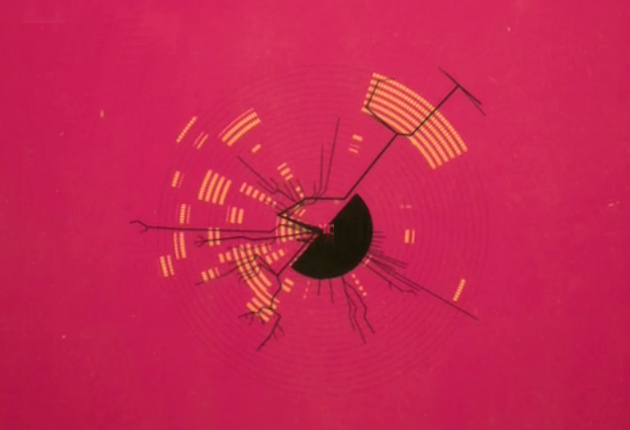
\includegraphics[width=6.00cm]{img/antivirus-flame-cyber-espace-renseignement-surveillance-stuxnet-doku.jpg}
\end{minipage}~\\

Complexit{\'e} jug{\'e}e sans pareille, nom flamboyant, attaques cibl{\'e}es contre certains int{\'e}r{\^e}ts gouvernementaux, Flame a tout d'une cyberarme nouvelle g{\'e}n{\'e}ration. Mais {\`a} y regarder de plus pr{\`e}s, Flame pourrait ne pas {\^e}tre aussi r{\'e}volutionnaire que certains m{\'e}dias et entreprises voudraient bien le laisser entendre.~\\

\textbf{L'alerte a {\'e}t{\'e} donn{\'e}e par Kaspersky~\footnote{\texttt{http://www.securelist.com/en/blog?weblogid=208193522}}}, un {\'e}diteur d'antivirus {\`a} la r{\'e}putation extr{\^e}mement solide. Flame serait le logiciel malveillant le plus complexe d{\'e}couvert {\`a} ce jour. \textbf{L'{\'e}diteur affirme~\footnote{\texttt{http://www.securelist.com/en/blog?weblogid=208193522}}} :~\\

	\textbf{\emph{Sa taille est importante, et il est incroyablement sophistiqu{\'e}. Il red{\'e}finit jusqu'{\`a} la notion m{\^e}me de cyberguerre et de cyberespionnage.}}~\\

Ses caract{\'e}ristiques si exceptionnelles... ne le sont cependant pas tant que \c{c}a. Flame est un cheval de Troie, {\`a} savoir un logiciel permettant {\`a} un attaquant de contr{\^o}ler un syst{\`e}me {\`a} l'insu de son utilisateur l{\'e}gitime via l'ex{\'e}cution d'un code malveillant. Quelles sont les fonctionnalit{\'e}s de Flame, selon Kaspersky ? Tout de ce qu'il y a de plus commun pour un malware que l'on trouve habituellement dans les milieux cybercriminels.~\\

En 2010, la d{\'e}couverte de Stuxnet changeait la donne en mati{\`e}re de cyberarme. Son perfectionnement d{\'e}passait les attentes. ...~\\

A savoir : la lecture, {\'e}criture et suppression de donn{\'e}es ; l'ex{\'e}cution de binaires ; la possibilit{\'e} de prendre des captures d'{\'e}cran ; l'enregistrement des frappes de clavier (keylogging) et la r{\'e}cup{\'e}ration et l'envoi de fichiers. D'autres fonctionnalit{\'e}s sont un peu plus recherch{\'e}es telles que l'enregistrement de donn{\'e}es audio (si microphone pr{\'e}sent) ou la possibilit{\'e} d'utiliser le bluetooth et le trafic r{\'e}seau pour r{\'e}cup{\'e}rer certaines informations sur l'environnement dans lequel est pr{\'e}sent l'ordinateur infect{\'e}.~\\

Des fonctionnalit{\'e}s, surprenantes et inqui{\'e}tantes pour un utilisateur lambda, en r{\'e}alit{\'e} extr{\^e}mement r{\'e}pandues depuis plus d'une dizaine d'ann{\'e}es. A titre d'exemple, le troyen Poison Ivy, dont la premi{\`e}re version date de 2005 et qui est toujours librement accessible sur Internet, offre la plupart des fonctionnalit{\'e}s de Flame, d{\'e}crites par Kaspersky comme constitutives de son originalit{\'e} ; et bien d'autres encore.~\\

{\`A} nos yeux, la seule originalit{\'e} de Flame, outre l'utilisation du \textbf{Lua~\footnotetext{\texttt{https://fr.wikipedia.org/wiki/Lua}}} [Un langage de script, NDLR] restreinte {\`a} une micro partie du corps du programme, concerne sa capacit{\'e} {\`a} utiliser le Bluetooth, bien qu'il ne soit fait mention nulle part de la possibilit{\'e} de se r{\'e}pandre via ce protocole. M{\^e}me ce qui est pr{\'e}sent{\'e} par Kaspersky comme la grande sp{\'e}cificit{\'e} de Flame, {\`a} savoir son fonctionnement en modules, n'est pas novatrice.~\\

De tr{\`e}s vieux troyens comme MiniMo, NuclearRAT, et bien s{\^u}r Poison Ivy fonctionnaient d{\'e}j{\`a} {\`a} partir d'un module principal d'infection auquel il {\'e}tait possible, une fois l'acc{\`e}s au syst{\`e}me effectif, d'ajouter diff{\'e}rents plug-ins selon l'utilisation que l'attaquant souhaitait faire de celui-ci (scanner distant, attaques DDoS, enregistrement de webcam, keylogging, etc.)... Flame, un p{\'e}tard mouill{\'e} ?~\\

\begin{minipage}[ht]{9.25cm}
	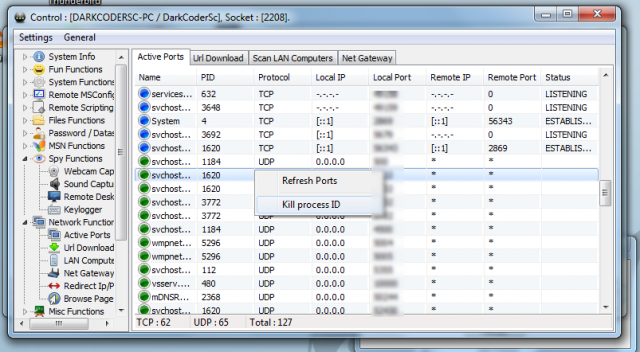
\includegraphics[width=9.00cm]{img/Flame-marketing-malware-e1338559312558.png}
\end{minipage} \hfill \begin{minipage}[ht]{9.50cm}
	\small
	Dans un article publi{\'e} \texttt{sur le site \emph{Atlantico}~\footnotemark}, l'expert en s{\'e}curit{\'e} informatique \texttt{Eric Filiol~\footnotemark} d{\'e}nonce le comportement de Kaspersky, et des {\'e}diteurs d'antivirus en g{\'e}n{\'e}ral, coupables {\`a} ses yeux de grossir certaines menaces dans le seul but de faire gonfler leur chiffre d'affaires.~\\

	En soi, cette th{\`e}se est recevable, et d'autant plus d'actualit{\'e} que les antivirus ont la tr{\`e}s mauvaise habitude de ne pas mettre {\`a} disposition les sources de leurs analyses. Cependant, trop occup{\'e} {\`a} {\'e}viter d'avaler la couleuvre de ce tr{\`e}s bel exemple d'utilisation marketing de la peur, M. Filiol tombe dans l'exc{\`e}s inverse, celui de la sous-estimation d'une menace peut-{\^e}tre r{\'e}elle. Les fonctionnalit{\'e}s de Flame que pr{\'e}sente Kaspersky ne sont pas nouvelles, et l'{\'e}diteur d'antivirus instrumentalise manifestement {\`a} son profit la faible connaissance qu'a l'utilisateur lambda de ce qui le menace sur Internet.~\\
\end{minipage}

~\footnotetext{\texttt{http://www.atlantico.fr/decryptage/virus-flame-kaspersky-peurs-occuper-terrain-mediatique-eric-filiol-375415.html}}
~\footnotetext{\texttt{http://fr.wikipedia.org/wiki/Eric\_Filiol}}

\textbf{\large Vieilles recettes}~\\

Que les fonctionnalit{\'e}s suppos{\'e}es de Flame \texttt{soient classiques~\footnote{http://www.securelist.com/en/blog?weblogid=208193522}} ne remet pas en question leur efficacit{\'e} ; les {\'E}tats utilisent des espions depuis la nuit des temps. Ce m{\^e}me sch{\'e}ma se retrouve dans le domaine du cyber-espionnage, des recettes identiques sont utilis{\'e}es depuis des ann{\'e}es (emails pi{\'e}g{\'e}s, r{\'e}cole d'information, pivot etc.) sans qu'il y ait de v{\'e}ritable r{\'e}volution. La soci{\'e}t{\'e} de \texttt{s{\'e}curit{\'e} RSA avait {\'e}t{\'e} pirat{\'e}e en 2011~\footnote{\texttt{http://www.securityvibes.fr/menaces-alertes/hack-rsa-details/}}} {\`a} l'aide de Poison Ivy, un RAT disponible sur Internet depuis plus d'une demi-d{\'e}cennie.~\\

Par ailleurs, nombreux ont {\'e}t{\'e} les experts informatiques {\`a} se gausser de la menace Flame en raison de sa taille importante (environ 20 Mo, tous plug-ins compris) ; m{\^e}me les plus vieux troyens g{\'e}n{\'e}raient des modules d'infection de quelques centaines de kilo-octets maximum, certains se contentant m{\^e}me avoisiner quelques Ko. Les d{\'e}veloppeurs de Flame seraient-il donc des <<amateurs>> ?~\\

Pas n{\'e}cessairement. Tout d'abord, car rien n'est dit de la possibilit{\'e} -- tr{\`e}s probable -- que Flame dispose, si ce n'est {\`a} la base, au moins d'un module rootkit. Les rootkits ont la particularit{\'e} de pouvoir cacher {\`a} peu pr{\`e}s tout ce qui se trouve sur un syst{\`e}me, des fichiers/dossiers aux processus, cl{\'e}s de registre et m{\^e}me le trafic passant par certains ports, qui pourrait indiquer {\`a} un observateur avis{\'e} que l'ordinateur se comporte d'une fa\c{c}on {\'e}trange. Or, si Flame est si complexe, et si, comme Kaspersky en fait mention, il a {\'e}t{\'e} capable d'infecter des syst{\`e}mes Windows 7 enti{\`e}rement patch{\'e}s, il est tr{\`e}s probable qu'il embarque des fonctionnalit{\'e}s de type Rootkit ou d'{\'e}l{\'e}vation de privil{\`e}ges non-connues publiquement. De plus, comme le dit tr{\`e}s justement F{\'e}lix Aim{\'e}, expert en s{\'e}curit{\'e} de l'information [{\'E}galement auteur sur Intel Strat, NDLR] :~\\

	\textbf{\emph{Qui donc v{\'e}rifie la taille des fichiers sur son disque dur pour en d{\'e}duire la pr{\'e}sence de virus ? La taille d'un virus n'a jamais {\'e}t{\'e} un indice de poids dans sa d{\'e}tection, c'est un mythe.}}~\\

Enfin, le dernier argument des experts sceptiques sur le cas Flame concerne la soi-disante violation d'un principe de base : <<un code, une cible>>. Bien {\'e}videmment, la r{\'e}ussite d'une attaque d{\'e}pend de sa planification et des informations qu'il a {\'e}t{\'e} possible de recueillir sur le syst{\`e}me-cible. Mais il est faux de penser qu'un attaquant va coder de A {\`a} Z un programme unique, exclusivement adapt{\'e} {\`a} une cible. S'il est vrai qu'un code malveillant se doit d'{\^e}tre adapt{\'e} aux sp{\'e}cificit{\'e}s du syst{\`e}me qu'il vise, un attaquant se contente g{\'e}n{\'e}ralement de moduler un code d{\'e}j{\`a} existant.~\\

Coder {\`a} usage unique n'est pas une pratique r{\'e}aliste et encore moins financi{\`e}rement viable. En fait, la structure en modules de Flame serait plut{\^o}t un argument appuyant sa dangerosit{\'e} ; peut-{\^e}tre m{\^e}me certains modules ont-ils {\'e}t{\'e} cod{\'e}s, {\`a} la base, pour une cible en particulier, et ont-ils {\'e}t{\'e} au fur et {\`a} mesure int{\'e}gr{\'e}s au fonctionnement global du malware.~\\

Flame ne r{\'e}d{\'e}finit pas la notion de cyberguerre, comme cela avait {\'e}t{\'e} pompeusement annonc{\'e}. La menace, en admettant qu'elle soit r{\'e}elle, n'en est pas pour atant dangereuse pour l'internaute lambda ; il est ici question d'un cheval de Troie, {\`a} la diffusion localis{\'e}e, et qui ne cible que des syst{\`e}mes appartenant {\`a} des personnalit{\'e}s strat{\'e}giques. Cependant, la multiplication de malwares si complexes qu'ils peuvent {\^e}tre consid{\'e}r{\'e}s comme de v{\'e}ritables cyberarmes confirme bien que les {\'E}tats investissent de plus en plus le cyberespace. Et prennent la mesure de son importance strat{\'e}gique.~\\

Article initialement publi{\'e} sur Intelligence-Strategique.eu~\footnote{\texttt{http://www.intelligence-strategique.eu/}} sous le titre : <<Stuxnet, Duqu, et maintenant Flame : course aux cyberarmes ou coup marketing ?~\footnote{http://www.intelligence-strategique.eu/2012/stuxnet-duqu-et-maintenant-flame-course-aux-cyberarmes-ou-coup-marketing/}>>~\\


%% \clearpage

\texttt{https://en.wikipedia.org/wiki/Stuxnet}~\\

%% \clearpage

\texttt{https://en.wikipedia.org/wiki/Duqu}~\\

%% \clearpage

\texttt{https://en.wikipedia.org/wiki/Flame\_(malware)}~\\


\clearpage

\texttt{http://www.intelligence-strategique.eu/2012/stuxnet-duqu-et-maintenant-flame-course-aux-cyberarmes-ou-coup-marketing/}~\\

\textbf{\LARGE Stuxnet, Duqu, et maintenant Flame : course aux cyberarmes ou coup marketing ?}~\\

\emph{\small Publi{\'e} le 01.06.2012 par Adrien G{\'e}vaudan}~\\

\lettrine{A}{bondamment trait{\'e}e dans nos colonnes}, la probl{\'e}matique de l'apparition de v{\'e}ritables cyberarmes semble conna{\^i}tre une nouvelle {\'e}volution avec l'annonce faite par l'{\'e}diteur d'antivirus Kaspersky de la d{\'e}couverte d'un nouveau malware, {\`a} la complexit{\'e} jug{\'e}e sans pareille, et flamboyeusement nomm{\'e} Flame. Toutefois, ce malware utilis{\'e} contre certains int{\'e}r{\^e}ts gouvernementaux et entreprises n'est pas aussi r{\'e}volutionnaire que le laissent entendre certains m{\'e}dias et entreprises.~\\

\textbf{\large Kaspersky : un whistle-blower en situation de conflit d'int{\'e}r{\^e}t}~\\

\texttt{L'alerte a {\'e}t{\'e} donn{\'e}e par Kaspersky~\footnote{\texttt{http://www.securelist.com/en/blog?weblogid=208193522}} }, un {\'e}diteur d'antivirus {\`a} la r{\'e}putation extr{\^e}mement solide (nombreux sont les experts {\`a} reconna{\^i}tre en sa suite de protection l'une des plus efficaces du secteur). Flame serait le malware le plus complexe d{\'e}couvert {\`a} ce jour. << Sa taille est importante, et il est incroyablement sophistiqu{\'e}. Il red{\'e}finit jusqu'{\`a} la notion m{\^e}me de cyberguerre et de cyberespionnage.~\footnotemark[10] >>, affirme l'{\'e}diteur. Ses caract{\'e}ristiques si exceptionnelles... ne le sont cependant pas tant que \c{c}a. En effet, nous sommes en pr{\'e}sence d'un cheval de Troie, {\`a} savoir un logiciel permettant {\`a} un attaquant de contr{\^o}ler un syst{\`e}me {\`a} l'insu de son utilisateur l{\'e}gitime via l'ex{\'e}cution d'un code malveillant. Quelles sont les fonctionnalit{\'e}s de Flame, selon Kaspersky ?~\\

\emph{Les fonctionnalit{\'e}s principales de Flame sont tout de ce qu'il y a de plus commun pour un malware que l'on trouve habituellement dans les milieux cybercriminels.}~\\

{`A} savoir : lecture, {\'e}criture et suppression de donn{\'e}es ; ex{\'e}cution de binaires ; possibilit{\'e} de prendre des captures d'{\'e}cran ; enregistrement des frappes de clavier (\emph{keylogging}). D'autres fonctionnalit{\'e}s sont un peu plus recherch{\'e}es telles que l'enregistrement de donn{\'e}es audio (si microphone pr{\'e}sent), la possibilit{\'e} d'utiliser le bluetooth et le trafic r{\'e}seau pour r{\'e}cup{\'e}rer certaines informations sur l'environnement dans lequel est pr{\'e}sent l'ordinateur infect{\'e}, ou encore la communication avec des serveurs de commande utilisant SSL vers des ports non-exotiques tels qu'HTTP (80), HTTPS (443) ou DNS (53) -- r{\'e}seau non domestique oblige.~\\

Et oui, il est possible de faire tout \c{c}a avec un programme informatique. Si cela peut para{\^i}tre surprenant et, {\`a} juste titre, inqui{\'e}tant {\`a} l'utilisateur d'ordinateur lambda, ces fonctionnalit{\'e}s sont en r{\'e}alit{\'e}... extr{\^e}mement r{\'e}pandues dans les \texttt{chevaux de Troie et autres RAT~\footnote{\texttt{http://en.wikipedia.org/wiki/Remote\_administration\_software}} }, et ce depuis plus d'une dizaine d'ann{\'e}es. A titre d'exemple, le troyen Poison Ivy, dont la premi{\`e}re version date de 2005 et qui est toujours librement accessible sur Internet, offre la plupart des fonctionnalit{\'e}s de Flame, d{\'e}crites par Kaspersky comme constitutives de son originalit{\'e} ; et bien d'autres encore.~\\

{`A} nos yeux, la seule originalit{\'e} de Flame, outre l'utilisation du \texttt{Lua~\footnote{\texttt{http://en.wikipedia.org/wiki/Lua\_(programming\_language)}}} restreinte {\`a} une micro partie du corps du programme, concerne sa capacit{\'e} {\`a} utiliser le Bluetooth, bien qu'il ne soit fait mention nulle part {\`a} la possibilit{\'e} de se r{\'e}pandre via ce protocole. M{\^e}me ce qui est pr{\'e}sent{\'e} par Kaspersky comme la grande sp{\'e}cificit{\'e} de Flame, {\`a} savoir son fonctionnement en modules, n'est absolument pas novatrice. De tr{\`e}s vieux troyens comme MiniMo ou NuclearRAT fonctionnaient d{\'e}j{\`a} {\`a} partir d'un module principal d'infection auquel il {\'e}tait possible, une fois l'acc{\`e}s au syst{\`e}me effectif, d'ajouter diff{\'e}rents plug-ins selon l'utilisation que l'attaquant souhaitait faire de celui-ci (scanner distant, attaques DDoS, enregistrement de webcam, keylogging, etc.)...~\\

Flame, un p{\'e}tard mouill{\'e} ?~\\

\begin{center}
	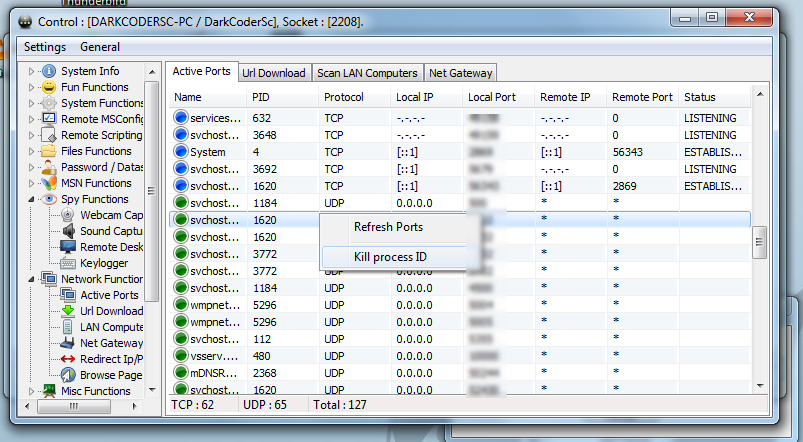
\includegraphics[width=16.00cm]{img/darkcomet.png}
	~\\ \emph{Darkcomet RAT -- Capture d'{\'e}cran du RAT DarkComet, d{\'e}velopp{\'e} par un fran\c{c}ais. }
\end{center}

\textbf{\large Entre marketing de la peur et menace r{\'e}elle} %% ~\\

Dans un article publi{\'e} \texttt{sur le site \emph{Atlantico}~\footnote{\texttt{http://www.atlantico.fr/decryptage/virus-flame-kaspersky-peurs-occuper-terrain-mediatique-eric-filiol-375415.html}}}, l'expert en s{\'e}curit{\'e} informatique \texttt{Eric Filiol~\footnote{\texttt{http://fr.wikipedia.org/wiki/Eric\_Filiol}}} d{\'e}nonce le comportement de Kaspersky, et des {\'e}diteurs d'antivirus en g{\'e}n{\'e}ral, coupables {\`a} ses yeux de grossir certaines menaces dans le seul but de faire gonfler leurs chiffres d'affaires. %% ~\\

--- En soi, cette th{\`e}se est parfaitement recevable, et d'autant plus d'actualit{\'e} que les antivirus ont la tr{\`e}s mauvaise habitude de ne jamais mettre {\`a} disposition les sources de leurs analyses. Cependant, trop occup{\'e} {\`a} {\'e}viter d'avaler la couleuvre de ce tr{\`e}s bel exemple d'utilisation marketing de la peur, M. Filiol tombe dans l'exc{\`e}s inverse, celui de la sous-estimation d'une menace peut-{\^e}tre r{\'e}elle. En effet, et comme nous l'avons dit, les fonctionnalit{\'e}s de Flame que nous pr{\'e}sente Kaspersky ne sont pas nouvelles, et il est manifeste que l'{\'e}diteur d'antivirus instrumentalise {\`a} son profit la faible connaissance qu'a l'utilisateur lambda de ce qui le menace sur Internet.~\\

\emph{Mais Flame pose une question cruciale en cyber-espionnage : est-il pertinent de juger de l'efficacit{\'e} d'une technique {\`a} l'aune de sa dur{\'e}e d'existence ?} %% ~\\

--- Que les fonctionnalit{\'e}s suppos{\'e}es de Flame soient classiques (toujours selon l'article de Kaspersky) ne remet pas en question leur efficacit{\'e} ; les Etats utilisent des espions depuis la nuit des temps, et il ne viendrait {\`a} personne l'id{\'e}e d'en contester l'efficacit{\'e} pour cette raison. Cela est tout {\`a} fait valable dans le domaine du cyber-espionnage, o{\`u} des recettes identiques sont utilis{\'e}es depuis des ann{\'e}es (emails pi{\'e}g{\'e}s, r{\'e}cole d'information, pivot etc.) sans qu'il y ait de v{\'e}ritable r{\'e}volution. La soci{\'e}t{\'e} de s{\'e}curit{\'e} RSA avait {\'e}t{\'e} pirat{\'e}e en 2011 {\`a} l'aide de Poison Ivy, un RAT disponible sur Internet depuis plus d'une demi-d{\'e}cennie.~\\

En outre, nombreux ont {\'e}t{\'e} les experts informatiques {\`a} se gausser de la menace Flame en raison sa taille importante (environ 20 Mo, tous plug-ins compris) ; en effet, m{\^e}me les plus vieux troyens g{\'e}n{\'e}raient des modules d'infection de quelques centaines de kilo-octets maximum, certains se contentant m{\^e}me d'avoisinner quelques Ko. Les d{\'e}veloppeurs de Flame seraient-il donc des << amateurs >> ? %% ~\\

--- Pas n{\'e}cessairement. Tout d'abord, car il n'est absolument pas fait mention de la possibilit{\'e} tr{\`e}s probable que Flame dispose, si ce n'est {\`a} la base, au moins d'un module rootkit. Les rootkits ont la particularit{\'e} de pouvoir cacher {\`a} peu pr{\`e}s tout ce qui se trouve sur un syst{\`e}me, des fichiers/dossiers aux processus, cl{\'e}s de registre et m{\^e}me le trafic passant par certains ports, qui pourrait indiquer {\`a} un observateur avis{\'e} que l'ordinateur se comporte d'une fa\c{c}on {\'e}trange. Or, si Flame est si complexe, et si, comme Kaspersky en fait mention, il a {\'e}t{\'e} capable d'infecter des syst{\`e}mes Windows 7 enti{\`e}rement patch{\'e}s, il est tr{\`e}s probable qu'il embarque des fonctionnalit{\'e}s de type Rootkit ou d'{\'e}levation de privil{\`e}ges non-connues publiquement. De plus, comme le dit tr{\`e}s justement F{\'e}lix Aim{\'e} : << Qui donc v{\'e}rifie la taille des fichiers sur son disque dur pour en d{\'e}duire la pr{\'e}sence de virus ? La taille d'un virus n'a jamais {\'e}t{\'e} un indice de poids dans sa d{\'e}tection, c'est un mythe. >>~\\

\emph{Il est parfaitement erron{\'e} de penser qu'un attaquant va coder de A {\`a} Z un programme unique, exclusivement adapt{\'e} {\`a} une cible.} %% ~\\

--- Enfin, le dernier argument des experts sceptiques sur le cas Flame concerne la soi-disante violation d'un principe de base : <<un code, une cible>>. Bien {\'e}videmment, la r{\'e}ussite d'une attaque d{\'e}pend de sa planification et des informations qu'il a {\'e}t{\'e} possible de r{\'e}cueillir sur le syst{\`e}me-cible. Mais il est parfaitement erron{\'e} de penser qu'un attaquant va coder de A {\`a} Z un programme unique, exclusivement adapt{\'e} {\`a} une cible. S'il est vrai qu'un code malveillant se doit d'{\^e}tre adapt{\'e} aux sp{\'e}cificit{\'e}s du syst{\`e}me qu'il vise, un attaquant se contente g{\'e}n{\'e}ralement de moduler un code d{\'e}j{\`a} existant. Coder {\`a} usage unique n'est pas une pratique r{\'e}aliste et encore moins financi{\`e}rement viable. En fait, la structure en modules de Flame serait plut{\^o}t un argument en faveur de sa s{\'e}riosit{\'e} ; peut-{\^e}tre m{\^e}me certains modules ont-ils {\'e}t{\'e} cod{\'e}s, {\`a} la base, pour une cible en particulier, et ont-ils {\'e}t{\'e} au fur et {\`a} mesure int{\'e}gr{\'e}s au fonctionnement global du malware.~\\

\textbf{\large Prudence, recul et esprit critique}~\\

D'un c{\^o}t{\'e}, nous avons donc un {\'e}diteur d'antivirus qui attire l'attention des utilisateurs sur un nouveau malware qu'il n'a pas d{\'e}cel{\'e} durant des ann{\'e}es, {\`a} la complexit{\'e} <<sans pr{\'e}c{\'e}dent>>, mais qui a tout int{\'e}r{\^e}t {\`a} l'apparition de tels programmes. De l'autre, une communaut{\'e} d'experts en s{\'e}curit{\'e}, sceptiques, questionnant la gravit{\'e} de la menace du troyen Flame, quand ce n'est pas son existence m{\^e}me ; mais qui se basent sur un comportement marketing pour contester une analyse technique, {\'e}cartant compl{\`e}tement la possibilit{\'e} que l'{\'e}diteur d'antivirus n'ait pas communiqu{\'e} la totalit{\'e} de ses informations. Le plus inqui{\'e}tant dans cette histoire reste la non d{\'e}tection par les diff{\'e}rents anti-virus de ce programme malveillant (d{\'e}couvert {\`a} l'origine par le CERT iranien) alors que c'est eux-m{\^e}me qui l'utilisent pour promouvoir leurs solutions de s{\'e}curit{\'e}...~\\

\emph{Aujourd'hui, au vu des donn{\'e}es disponibles, force est de constater que Flame ne r{\'e}d{\'e}finit pas la notion m{\^e}me de cyberguerre, comme cela avait {\'e}t{\'e} pompeusement annonc{\'e}.} %% ~\\

--- Il convient de toujours porter un regard critique sur les informations que peuvent communiquer des entreprises ayant directement int{\'e}r{\^e}t {\`a} ce qu'on les diffuse, encore plus lorsqu'elles ne proviennent que d'une source unique. Mais il est {\'e}galement n{\'e}cessaire de ne pas tomber dans l'exc{\`e}s de m{\'e}fiance, et rejeter toute information sous pr{\'e}texte qu'elle est issue d'une entreprise qui, par essence, cherche {\`a} maximiser son profit.~\\

Aujourd'hui, au vu des donn{\'e}es disponibles, force est de constater que Flame ne r{\'e}d{\'e}finit pas la notion m{\^e}me de cyberguerre, comme cela avait {\'e}t{\'e} pompeusement annonc{\'e}. La menace, en admettant qu'elle soit r{\'e}elle, n'en est pas pour autant dangereuse pour l'internaute lambda ; il est ici question d'un cheval de Troie, {\`a} la diffusion localis{\'e}e, et qui ne cible que des syst{\`e}mes appartenant {\`a} des personnalit{\'e}s strat{\'e}giques. Au final, la multiplication de malwares si complexes qu'ils peuvent {\^e}tre consid{\'e}r{\'e}s comme de v{\'e}ritables cyberarmes confirme bien que les Etats prennent peu {\`a} peu la mesure de l'importance strat{\'e}gique de disposer de capacit{\'e}s d'action dans le cyberespace.~\\

\textbf{\emph{\large Cyber-espionnage : deux orientations dans le d{\'e}veloppement de malwares. }}~\\

\emph{Avec l'apparition de Duqu et de Flame, nous pouvons discerner deux orientations strat{\'e}giques concernant le d{\'e}veloppement de malwares utilis{\'e}s dans des op{\'e}rations de cyber-espionnage.}~\\

\emph{Lors d'attaques APT (Advanced Persistent Threat) dont sont victimes principalement les entreprises et gouvernements occidentaux, un simple malware (souvent r{\'e}pandu sur Internet, tel que Poison Ivy) est ex{\'e}cut{\'e} sur un ordinateur interne au r{\'e}seau cibl{\'e}. Une fois ex{\'e}cut{\'e}, les op{\'e}rateurs derri{\`e}re l'attaque d{\'e}ploient plusieurs autres logiciels malveillants avec pour chacun deux leurs sp{\'e}cificit{\'e}s afin d'{\'e}lever leurs privil{\`e}ges sur une partie ou l'ensemble du r{\'e}seau, devenant {\`a} terme administrateur du \texttt{contr{\^o}leur de domaine~\footnote{\texttt{http://fr.wikipedia.org/wiki/Active\_Directory}} } (le coeur du r{\'e}seau).}~\\

\emph{Parrall{\`e}lement {\`a} ces attaques, une autre strat{\'e}gie privil{\'e}gie des malwares d{\'e}velopp{\'e}s sous forme de modules o{\`u} chacun d'eux est destin{\'e} {\`a} une t{\^a}che pr{\'e}cise. Cette deuxi{\`e}me strat{\'e}gie {\`a} l'air d'{\^e}tre uniquement adopt{\'e}e lors d'attaques ciblant le Moyen et le Proche Orient, th{\'e}{\^a}tre de conflits li{\'e}s principalement {\`a} la puissance iranienne.}~\\

\clearpage

\texttt{http://www.lemonde.fr/international/article/2012/08/15/le-pentagone-veut-porter-la-cyberguerre-hors-des-etats-unis\_1746263\_3210.html}~\\

\textbf{\LARGE Le Pentagone veut porter la cyberguerre hors des Etats-Unis}~\\

\emph{\small LE MONDE | 15.08.2012 {\`a} 11h52 -- Mis {\`a} jour le 15.08.2012 {\`a} 14h08}~\\

Par Sylvain Cypel (New York, correspondant)~\\

\begin{minipage}[ht]{12.25cm}
	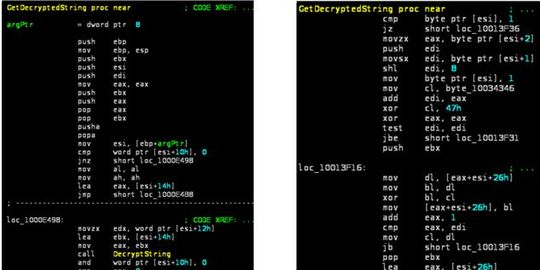
\includegraphics[width=12.00cm]{img/1744629_3_8bd2_les-virus-flame-et-gauss-sont-assez-similaires_6da5f9190191e99b3ac718154775b7f0.jpg}
	~\\ \emph{\centering Les virus Flame et Gauss sont assez similaires. }
\end{minipage} \hfill \begin{minipage}[ht]{6.50cm}
	\small
	Le Pentagone n'a fait aucun commentaire depuis la r{\'e}v{\'e}lation, la semaine derni{\`e}re, de nouvelles cyberattaques, men{\'e}es surtout dans le milieu bancaire libanais, par un puissant virus que son d{\'e}couvreur, la soci{\'e}t{\'e} de s{\'e}curit{\'e} informatique russe Kaspersky Lab, a nomm{\'e} "Gauss".~\\
	
	En revanche, le Pentagone fait pression sur le Congr{\`e}s pour qu'il autorise l'adoption de nouvelles normes permettant {\`a} l'arm{\'e}e et aux agences sp{\'e}cialis{\'e}es des Etats-Unis d'user de moyens plus "offensifs", en particulier de mener des cyberattaques contre des objectifs {\`a} l'{\'e}tranger.~\\
\end{minipage}~\\

Le principal instigateur de cette revendication est le g{\'e}n{\'e}ral Keith Alexander, chef du Cyber Command, une unit{\'e} sp{\'e}ciale cr{\'e}{\'e}e il y a deux ans. Actuellement, la d{\'e}fense am{\'e}ricaine n'est autoris{\'e}e qu'{\`a} prot{\'e}ger son propre territoire contre des cyberattaques. --- Le g{\'e}n{\'e}ral souhaite que ses r{\`e}gles op{\'e}rationnelles soient modifi{\'e}es afin de pouvoir entreprendre des actions "\emph{raisonnables et proportionn{\'e}es}" hors du territoire am{\'e}ricain en cas de "\emph{menace imminente contre les Etats-Unis}". --- Ce sujet est d{\'e}battu depuis plusieurs mois par les plus hautes instances de l'Etat am{\'e}ricain : d{\'e}fense, affaires {\'e}trang{\`e}res, justice et Tr{\'e}sor.~\\

Les banques et le secteur financier ne sont pas les moins concern{\'e}s, par exemple dans le domaine du suivi des sanctions internationales contre l'Iran ou celui des mouvements de fonds soup\c{c}onn{\'e}s d'{\^e}tre li{\'e}s au terrorisme et au blanchiment, comme l'a montr{\'e} la r{\'e}cente affaire de la banque HSBC, qui a admis avoir effectu{\'e} 25 000 transactions suspectes avec l'Iran entre 2001 et 2007 pour 19,4 milliards de dollars (15,7 milliards d'euros).~\\

Mardi 14 ao{\^u}t, une autre banque britannique, Standard Chartered, a vers{\'e} 240 millions de dollars d'amende pour mettre fin {\`a} toutes poursuites des services financiers de l'Etat de New York, qui l'accusaient de transactions illicites avec T{\'e}h{\'e}ran, portant sur 250 milliards de dollars.~\\

\textbf{EVITER DES BAVURES}~\\

Le secteur bancaire est le plus vis{\'e} par le virus Gauss, qui, selon les experts, "\emph{sort avec une tr{\`e}s haute probabilit{\'e} du ou des m{\^e}mes usines}" -- r{\'e}f{\'e}rence implicite aux Etats-Unis et {\`a} Isra{\"e}l. Gauss se serait principalement attaqu{\'e} {\`a} des banques situ{\'e}es au Liban, o{\`u} 1 660 ordinateurs auraient {\'e}t{\'e} cibl{\'e}s (734 l'auraient aussi {\'e}t{\'e} en Isra{\"e}l et en Palestine, et 43 aux Etats-Unis).~\\

Les banques cit{\'e}es sont Byblos, Cr{\'e}dit libanais et Blombank, mais les am{\'e}ricains Citibank et PayPal (le syst{\`e}me de paiement du site commercial en ligne eBay) auraient {\'e}galement vu leurs syst{\`e}mes informatiques espionn{\'e}s ou endommag{\'e}s. --- Jeffrey Carr, cr{\'e}ateur de la soci{\'e}t{\'e} de cybers{\'e}curit{\'e} Taia Global, soup\c{c}onne des op{\'e}rations "\emph{visant le Hezbollah}", d'autres {\'e}voquent les liens iraniens ou syriens avec la finance libanaise.~\\

Cette cyberguerre se m{\`e}ne en secret. Mais, pour l{\'e}gif{\'e}rer, comment et quand d{\'e}finir la r{\'e}alit{\'e} de la menace ? La justice et le d{\'e}partement d'Etat am{\'e}ricains souhaitent {\'e}viter des bavures, en particulier dans des actions amen{\'e}es {\`a} viser le territoire de "\emph{pays alli{\'e}s}". --- Le lobby financier, lui, tente de freiner au Congr{\`e}s toute vell{\'e}it{\'e} d'imposer une tra\c{c}abilit{\'e} des transactions {\'e}lectroniques.~\\

\emph{\small Sylvain Cypel (New York, correspondant)} %% ~\\

\clearpage

\texttt{http://www.lemonde.fr/technologies/article/2012/08/09/le-virus-gauss-vise-des-transactions-bancaires-au-moyen-orient\_1744625\_651865.html}~\\

\textbf{\LARGE Le virus Gauss vise des transactions bancaires au Moyen-Orient}~\\

\emph{\small Le Monde.fr avec AFP | 09.08.2012 {\`a} 20h16 -- Mis {\`a} jour le 10.08.2012 {\`a} 08h50}~\\

\begin{minipage}[ht]{12.25cm}
	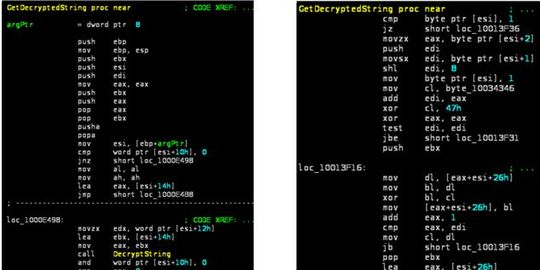
\includegraphics[width=12.00cm]{img/1744629_3_8bd2_les-virus-flame-et-gauss-sont-assez-similaires_6da5f9190191e99b3ac718154775b7f0.jpg}
	~\\ \emph{\centering Les virus Flame et Gauss sont assez similaires. }
\end{minipage} \hfill \begin{minipage}[ht]{6.50cm}
	\small 
	Un nouveau virus informatique, baptis{\'e} Gauss et pr{\'e}sentant des similarit{\'e}s avec Flame et Stuxnet, a {\'e}t{\'e} con\c{c}u pour espionner les transactions bancaires en ligne, a annonc{\'e} jeudi 9 ao{\^u}t la soci{\'e}t{\'e} russe Kaspersky Lab, qui pr{\'e}cise que des donn{\'e}es de banques libanaises ont {\'e}t{\'e} pirat{\'e}es.~\\
	
	Selon le sp{\'e}cialiste de la lutte antivirus, Gauss est un "\emph{kit complet d'outils de cyberespionnage}" cr{\'e}{\'e} par un Etat, sans pr{\'e}ciser lequel. Ce "\emph{cheval de Troie visant la banque en ligne}" permet de voler les mots de passe, les identifiants de comptes bancaires et de pirater les modes de paiement en ligne, pr{\'e}cise Kaspersky dans un communiqu{\'e}.~\\
\end{minipage}

\textbf{GAUSS NE VISE PAS L'IRAN MAIS LE LIBAN}~\\

Op{\'e}rationnel depuis septembre 2011, il a {\'e}t{\'e} d{\'e}couvert en juin "\emph{gr{\^a}ce aux enseignements tir{\'e}s de l'{\'e}tude approfondie men{\'e}e sur Flame}", explique la soci{\'e}t{\'e}. "\emph{Gauss pr{\'e}sente des ressemblances frappantes avec Flame, telles que sa conception et son code source, ce qui nous a permis de le d{\'e}couvrir}", affirme l'expert en chef de la s{\'e}curit{\'e} de Kaspersky, Alexander Gostev, cit{\'e} dans le communiqu{\'e}.~\\

"\emph{Une autre sp{\'e}cificit{\'e} de Gauss tient {\`a} sa capacit{\'e} {\`a} infecter les cl{\'e}s USB via la m{\^e}me vuln{\'e}rabilit{\'e} pr{\'e}c{\'e}demment exploit{\'e}e par Stuxnet et Flame}", note la soci{\'e}t{\'e} russe. Mais l{\`a} o{\`u} Stuxnet et Flame visaient l'Iran, Gauss semble s'attaquer {\`a} des banques libanaises, notamment Bank of Beirut, EBLOF, BlomBank, ByblosBank ou encore le Cr{\'e}dit libanais. Le virus a par ailleurs cibl{\'e} des utilisateurs de Citibank et de PayPal, ajoute Kaspersky qui estime {\`a} 2 500 le nombre d'ordinateurs infect{\'e}s, contre 700 pour Flame.~\\

Selon le \emph{New York Times}, le pr{\'e}sident am{\'e}ricain Barack Obama est {\`a} l'origine d'une augmentation des cyberattaques contre le programme nucl{\'e}aire iranien et le virus Flame serait, si l'on en croit le \emph{Washington Post}, le produit d'une collaboration entre les agences am{\'e}ricaines de renseignement et l'arm{\'e}e isra{\'e}lienne.~\\


\end{document}
